% !TeX program = lualatex
% Der sehende Stein - LaTeX Testprojekt
% Compiler: LuaLaTeX (auch pdfLaTeX moeglich)
\documentclass[11pt,a4paper,twoside]{book}
\usepackage[ngerman]{babel}
\usepackage[T1]{fontenc}
\usepackage[utf8]{inputenc}
\usepackage{lmodern}
\usepackage{microtype}
\usepackage{xcolor}
\usepackage{graphicx}
\usepackage{geometry}
\geometry{inner=24mm,outer=19mm,top=23mm,bottom=23mm}
\usepackage{multicol}
\usepackage[most]{tcolorbox}
\usepackage{fancyhdr}
\usepackage{titlesec}
\usepackage{hyperref}
\usepackage{lettrine}
\definecolor{ink}{HTML}{292923}
\definecolor{wine}{HTML}{68332E}
\definecolor{parchment}{HTML}{F5F0E5}
\definecolor{oldgold}{HTML}{92764F}
\color{ink}
\hypersetup{colorlinks=true,linkcolor=wine,pdfauthor={Jörg Jacob mit ChatGPT},pdftitle={Der sehende Stein -- Ein Cthulhu-Abenteuer}}
\pagestyle{fancy}
\fancyhf{}
\fancyhead[LE,RO]{\footnotesize\sffamily DER SEHENDE STEIN}
\fancyhead[LO,RE]{\footnotesize\sffamily DER SEHENDE STEIN}
\fancyfoot[C]{\thepage}
\renewcommand{\headrulewidth}{0.3pt}
\titleformat{\chapter}[display]{\normalfont\Huge\bfseries\color{wine}}{}{0pt}{}[\vspace{2mm}\titlerule]
\titlespacing*{\chapter}{0pt}{0pt}{16pt}
\titleformat{\section}{\Large\bfseries\color{wine}}{}{0pt}{}
\titleformat{\subsection}{\large\bfseries\color{wine}}{}{0pt}{}
\newtcolorbox{vorlesetext}{enhanced,breakable,colback=parchment,colframe=oldgold,boxrule=.7pt,arc=1mm,left=10pt,right=10pt,top=9pt,bottom=9pt,before skip=12pt,after skip=12pt,title={\sffamily\bfseries VORLESETEXT --- KARIM EL-MADY (JÖRG)},colbacktitle=oldgold,coltitle=white,fonttitle=\footnotesize}
\newtcolorbox{vorlesetextalle}{enhanced,breakable,colback=parchment,colframe=oldgold,boxrule=.7pt,arc=1mm,left=10pt,right=10pt,top=9pt,bottom=9pt,before skip=12pt,after skip=12pt,title={\sffamily\bfseries VORLESETEXT --- AN ALLE VIER SPIELER},colbacktitle=oldgold,coltitle=white,fonttitle=\footnotesize}
\newtcolorbox{meisterinfo}{enhanced,breakable,colback=white,colframe=wine,boxrule=.6pt,arc=1mm,left=10pt,right=10pt,top=8pt,bottom=8pt,title={\sffamily\bfseries HINWEISE FÜR DIE SPIELLEITUNG},colbacktitle=wine,coltitle=white,fonttitle=\footnotesize}
\setlength{\parindent}{1em}
\setlength{\parskip}{3pt}
\begin{document}
\begin{titlepage}
\centering
\vspace*{20mm}
{\large\sffamily EIN ABENTEUER FÜR DAS CTHULHU-ROLLENSPIEL\par}
\vspace{15mm}
{\Huge\bfseries\color{wine} Der sehende Stein\par}
\vspace{4mm}
{\Large Akt I und II -- Arkham und Ägypten\par}
\vspace{19mm}

\includegraphics[width=0.33\textwidth,keepaspectratio]{bilder/miskatonic-siegel.png}\par
\vspace{19mm}
{\Large Akt I: Arkham $\circ$ Akt II: Ägypten\par}
\vspace{4mm}
{\large Akt I: Szenen 1 bis 3 und Akt II: Szenen 1 bis 5 und Epilog\par}
\vfill
{\sffamily\small ARBEITSFASSUNG $\circ$ 29. OKTOBER 2026\par}
{\sffamily\footnotesize Interne Arbeitsfassung -- nicht zur Veröffentlichung\par}
\end{titlepage}
\tableofcontents
\clearpage
\chapter{Die Schatten von Arkham}
\section{Der Auftrag der Miskatonic University}
\subsection{1.1 -- Ankunft auf dem Universitätsgelände}
\noindent\textbf{Ort:} Miskatonic University, Arkham, Massachusetts\\
\textbf{Zeit:} 5. April 1920, etwa 10 Uhr morgens\\
\textbf{Im Mittelpunkt:} Karim el-Mady (Jörg)


\begin{figure}[htbp]
\centering
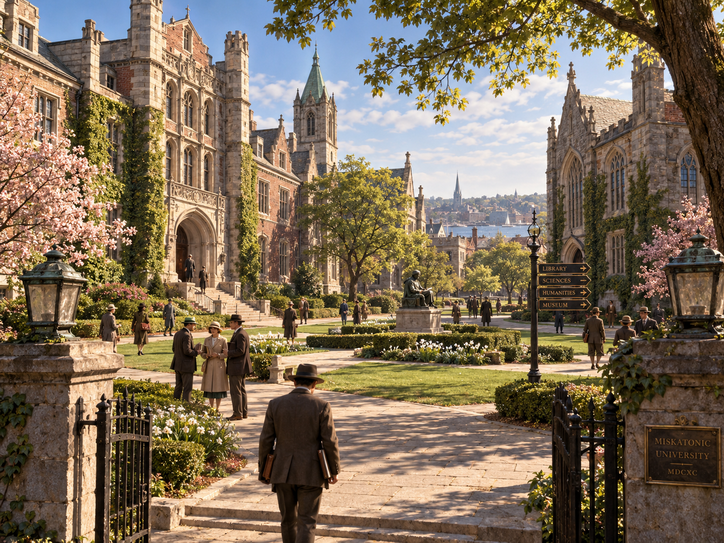
\includegraphics[width=\textwidth]{bilder/miskatonic-campus-im-fruehling.png}
\caption{Die Miskatonic University an einem sonnigen Frühlingsvormittag in Arkham.}
\end{figure}

\begin{vorlesetext}
Es ist ein herrlicher Vormittag in Arkham. Die Sonne steht bereits hoch am nahezu wolkenlosen Himmel und taucht das weitläufige Gelände der altehrwürdigen Miskatonic University in ein warmes, goldenes Licht. Eine leichte Brise bewegt die Blätter der mächtigen Laubbäume, die seit Generationen über die Wege und Grünanlagen des Universitätsgeländes wachen.

Vor Dir erstreckt sich ein beeindruckendes Ensemble ehrwürdiger Bauwerke. Gewaltige Fassaden aus grauem und rötlichem Naturstein erheben sich über sorgfältig angelegten Rasenflächen. Hohe, schmale Fenster mit steinernen Einfassungen durchbrechen die massiven Mauern, während aufwendig gearbeitete Gesimse, Rundbögen und verwitterte Ornamente von der langen Geschichte der Universität zeugen. An manchen Gebäuden rankt sich dichter Efeu bis hinauf zu den oberen Stockwerken. Über den Dächern ragen vereinzelt schlanke Türmchen und reich verzierte Giebel empor.

Trotz ihres beträchtlichen Alters wirken die Gebäude au\ss{}erordentlich gepflegt. Die Fenster glänzen im Sonnenlicht, die steinernen Treppenaufgänge sind sauber gefegt, und selbst die ältesten Mauern strahlen eine gewisse Würde und Beständigkeit aus. Es ist die Art von Ort, an dem man unwillkürlich die Stimme ein wenig senkt, als wolle man die Gelehrsamkeit vergangener Jahrhunderte nicht stören.

Breite, mit hellen Steinplatten gepflasterte Wege durchziehen den Campus und verbinden die zahlreichen Fakultätsgebäude miteinander. Dazwischen liegen kleine, von Blumenrabatten eingefasste Plätze, gepflegte Hecken und schattige Sitzgelegenheiten unter alten Bäumen.

Das Universitätsleben ist bereits in vollem Gange. Junge Männer und Frauen eilen mit Büchern, Ledermappen und zusammengerollten Schriftstücken unter den Armen über die Wege. Einige tragen einfache Kleidung, andere wirken in ihren tadellos sitzenden Anzügen und vornehmen Kleidern beinahe ebenso ehrwürdig wie die Gebäude selbst. Vor einem der gro\ss{}en Eingangsportale stehen drei ältere Herren in dunklen Anzügen beisammen, offenbar in eine angeregte Diskussion vertieft. Einer von ihnen gestikuliert mit einer Pfeife, während die beiden anderen aufmerksam zuhören.

Von einer nahe gelegenen Turmuhr schlägt es zehn.

Du bleibst für einen Augenblick stehen und lässt Deinen Blick über das geschäftige Treiben schweifen. Die Wege verzweigen sich in mehrere Richtungen, führen vorbei an weiteren Gebäuden, durch kleine Grünanlagen und über offene Plätze. An verschiedenen Wegkreuzungen stehen schmiedeeiserne Wegweiser mit sorgfältig beschrifteten Tafeln. Vereinzelt sind an den Eingängen der Gebäude steinerne Schilder und Wappen angebracht.

Irgendwo auf diesem weitläufigen Campus befindet sich das Verwaltungsgebäude, in dem Du um elf Uhr einen Termin beim Präsidenten der Universität hast.

Noch bleibt Dir genügend Zeit, Dich zurechtzufinden.
\end{vorlesetext}

\begin{meisterinfo}
\textbf{Ziel der Szene.} Karim soll eigenständig den Weg zum Verwaltungsgebäude finden. Die Szene gibt ihm etwas Raum, seine Figur kennenzulernen und erste Entscheidungen zu treffen.

\medskip\noindent\textbf{Mögliche Vorgehensweisen:}
\begin{itemize}
\item \textbf{Beschilderung folgen:} Bei näherer Betrachtung der Wegweiser findet Karim Hinweise auf das Verwaltungsgebäude. Keine Fertigkeitsprobe nötig.
\item \textbf{Studierende ansprechen:} Ein vorbeieilender Student kann ihm den Weg erklären -- vielleicht etwas gehetzt, aber höflich.
\item \textbf{Lehrkräfte ansprechen:} Einer der älteren Herren gibt bereitwillig Auskunft und könnte sich nach dem Anlass des Besuchs erkundigen.
\item \textbf{Auf eigene Faust suchen:} Karim kann einen Weg einschlagen; gegebenenfalls gelangt er über einen kleinen Umweg zum richtigen Gebäude.
\end{itemize}

\textbf{Atmosphäre.} Der Einstieg soll ruhig und freundlich wirken. Noch deutet nichts auf das Grauen hin. Die Universität erscheint als Ort der Wissenschaft, Ordnung und Sicherheit.

\textbf{Szenenabschluss.} Frage den Spieler: \emph{\glqq{}Was möchtest Du tun?\grqq{}} 
\end{meisterinfo}

\noindent\textit{Redaktioneller Hinweis: Die Handlung ist derzeit für den 5. April 1920 angesetzt. Der ungewöhnlich warme, fast sommerliche Eindruck wird bewusst als sonniger Frühlingstag beschrieben.}

\clearpage
\section{Vor dem Verwaltungsgebäude}
\label{sec:verwaltung-aussen}
\noindent\textbf{Abschnitt:} 1.2\quad
\textbf{Ort:} Veranda des Verwaltungsgebäudes\quad
\textbf{Zeit:} 5. April 1920, gegen 10 Uhr

\begin{center}
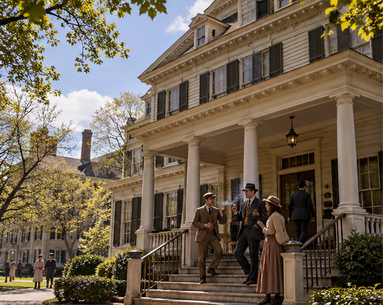
\includegraphics[width=.94\textwidth]{bilder/verwaltungsgebaeude-aussen.png}
\par\vspace{3pt}{\footnotesize\itshape Das Verwaltungsgebäude der Miskatonic University mit seiner gro\ss{}zügigen Veranda.}
\end{center}

\begin{vorlesetext}
Nach einem kurzen Spaziergang über die gepflegten Wege des Universitätsgeländes gelangst Du an einen kleinen, von alten Laubbäumen gesäumten Platz. Vor Dir erhebt sich ein stattliches, dreistöckiges Gebäude, das sich in seiner Architektur deutlich von den gewaltigen steinernen Fakultätsgebäuden unterscheidet.

Das Haus ist ganz im Stil der traditionellen amerikanischen Architektur gehalten. Seine breite Fassade besteht aus sorgfältig verarbeiteten, horizontal angebrachten Holzbrettern, deren ursprünglich cremewei\ss{}er Anstrich im hellen Sonnenlicht beinahe makellos erscheint. Hohe, regelmä\ss{}ig angeordnete Sprossenfenster mit dunkelgrünen Fensterläden verleihen dem Gebäude eine gewisse Strenge, die jedoch durch die gro\ss{}zügigen Proportionen und die zahlreichen architektonischen Verzierungen aufgelockert wird. Ein steiles, mit dunklen Schindeln gedecktes Dach schlie\ss{}t das oberste Geschoss ab. Mehrere gemauerte Schornsteine ragen darüber hinaus.

Eine breite, überdachte Veranda erstreckt sich über nahezu die gesamte Vorderseite des Hauses. Schlanke, wei\ss{} gestrichene Holzsäulen tragen das leicht geneigte Vordach. Zwischen ihnen verläuft ein aufwendig gearbeitetes Geländer, an dessen Fu\ss{} einige gro\ss{}e Terrakottatöpfe mit blühenden Pflanzen aufgestellt sind. Eine breite Holztreppe mit fünf flachen Stufen führt von dem gepflasterten Vorplatz hinauf zur Veranda.

Dort stehen drei junge Leute, zwei Herren und eine Dame, die sich offenbar angeregt unterhalten. Einer der Herren lehnt mit lässig verschränkten Beinen an einer der wei\ss{}en Säulen und hält eine brennende Zigarette zwischen den Fingern. Sein Begleiter, in einem hellbraunen Anzug und mit etwas zerzaustem Haar, gestikuliert lebhaft, während die junge Dame mit einem amüsierten Lächeln zuhört. Hin und wieder steigt eine dünne, bläuliche Rauchfahne empor, die sich langsam unter dem Verandadach verliert.

Das gedämpfte Knarren der hölzernen Dielen mischt sich mit ihren Stimmen und dem fernen Treiben des Campus. Als Du näher kommst, wendet einer der jungen Männer kurz den Kopf in Deine Richtung, schenkt Dir ein höfliches Nicken und setzt sein Gespräch fort.

Hinter der kleinen Gruppe befindet sich eine breite, dunkel lackierte Eingangstür mit zwei verglasten Flügeln. Das blank polierte Messing der Türgriffe glänzt im Sonnenlicht.
\end{vorlesetext}

\begin{meisterinfo}
\textbf{Situation.} Karim kann die Gruppe ansprechen, das Gebäude näher betrachten oder direkt eintreten. Eine Fertigkeitsprobe ist nicht erforderlich. Die drei Studierenden machen eine kurze Pause zwischen Veranstaltungen. Sie sind höflich, aber mit ihrem Gespräch beschäftigt.

\medskip
\textbf{Frage: Ist dies das Verwaltungsgebäude?}

\emph{\glqq{}Ja, ganz richtig. Hier sind Sie bei der Verwaltung. Wenn Sie jemanden suchen, wenden Sie sich am besten gleich an den Empfang. Direkt hinter der Eingangstür, Sie können ihn gar nicht verfehlen.\grqq{}}

\medskip
\textbf{Frage: Wo ist der Universitätspräsident?}

\emph{\glqq{}Zum Präsidenten? Dann haben Sie jedenfalls das richtige Gebäude gefunden. Sein Büro liegt irgendwo oben. Der Herr am Empfang wird Ihnen sicher weiterhelfen können.\grqq{}}

\medskip
\textbf{Frage: Muss ich mich anmelden?}

\emph{\glqq{}Das würde ich Ihnen empfehlen. Die Herren hier legen ziemlich gro\ss{}en Wert auf solche Dinge.\grqq{}}

\medskip
\textbf{Frage: Kennen Sie Professor Garmond?}

\emph{\glqq{}Professor Garmond? Ein vielbeschäftigter Mann. Man bekommt ihn nicht gerade häufig zu Gesicht. Aber wenn Sie einen Termin haben, werden Sie wohl schon erwartet.\grqq{}}

\medskip
\textbf{Grenze ihres Wissens.} Die Studierenden wissen nichts über die verschwundene Expedition. Bei weiteren Fragen verweisen sie auf den Empfang.

\textbf{Übergang.} Sobald Karim die Eingangstür öffnet, beginnt Abschnitt 1.3.
\end{meisterinfo}

\clearpage
\section{Die Eingangshalle der Universitätsverwaltung}
\label{sec:verwaltung-innen}
\noindent\textbf{Abschnitt:} 1.3\quad
\textbf{Ort:} Eingangshalle und Empfang\quad
\textbf{Zeit:} 5. April 1920, gegen 10 Uhr

\begin{center}
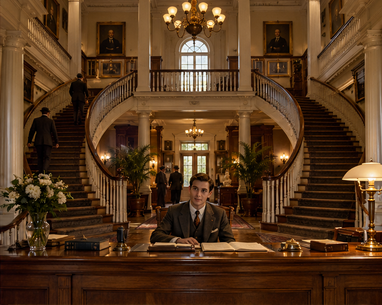
\includegraphics[width=.94\textwidth]{bilder/verwaltung-eingangshalle.png}
\par\vspace{3pt}{\footnotesize\itshape Die Eingangshalle mit dem Empfangstresen zwischen den beiden Treppenaufgängen.}
\end{center}

\begin{vorlesetext}
Du drückst einen der schweren Messinggriffe herunter und öffnest die Eingangstür. Mit einem leisen Knarren schwingt der Türflügel nach innen, und Du trittst über die Schwelle.

Du findest Dich in einer überraschend gro\ss{}en, lichtdurchfluteten Halle wieder. Die hohen Decken und gro\ss{}zügigen Abmessungen des Raumes lassen das Gebäude von innen noch eindrucksvoller erscheinen, als es von au\ss{}en ohnehin schon gewirkt hat.

Der Boden besteht aus gro\ss{}en, hellgrauen Natursteinplatten, die sorgfältig geschliffen wurden und im einfallenden Tageslicht einen matten Glanz zeigen. Ein breiter, dunkelroter Teppichläufer führt vom Eingangsbereich geradewegs zu einem mächtigen Empfangstresen aus dunkel gebeiztem Eichenholz.

Links und rechts erheben sich zwei breite, elegant geschwungene Holztreppen. Ihre polierten Geländer folgen in weiten Bögen den Treppenläufen hinauf zu einer offenen Galerie im ersten Obergeschoss, von der aus weitere Treppen in die darüberliegenden Stockwerke führen. Die Treppenstufen sind mit schmalen Teppichläufern belegt, die von blanken Messingstangen gehalten werden.

Die Wände der Halle sind im unteren Bereich mit dunklem Holz vertäfelt. Darüber hängen mehrere gro\ss{}e Ölgemälde in schweren, vergoldeten Rahmen, die würdevoll dreinblickende Herren in akademischer Kleidung zeigen. Vermutlich frühere Präsidenten oder andere bedeutende Persönlichkeiten der Universität.

Ein mächtiger Kronleuchter aus Messing und geschliffenem Glas hängt von der hohen Decke herab. Obwohl seine elektrischen Lampen nicht eingeschaltet sind, fällt durch die hohen Fenster genügend Sonnenlicht in den Raum, um selbst die entferntesten Winkel zu erhellen.

Hinter dem Empfangstresen sitzt ein junger Mann von vielleicht fünfundzwanzig Jahren. Er trägt einen tadellos sitzenden dunkelgrauen Anzug, eine schmale Krawatte und eine sorgfältig frisierte, seitlich gescheitelte Frisur. Neben ihm stehen ein Telefonapparat mit getrenntem Hörer, mehrere Ablagekörbe und ein kleiner Stapel Schriftstücke.

Als Du eintrittst, ist er gerade damit beschäftigt, einige Eintragungen in einem gro\ss{}en, ledergebundenen Buch vorzunehmen. Er führt seinen Füllfederhalter mit schnellen, geübten Bewegungen über das Papier.

Beim Geräusch der zufallenden Eingangstür hält er inne. Er legt den Füllfederhalter sorgfältig neben das aufgeschlagene Buch, hebt den Kopf und blickt Dir mit einem freundlichen, aber professionellen Lächeln entgegen.
\end{vorlesetext}

\begin{meisterinfo}
\textbf{Empfangsmitarbeiter.} Der junge Angestellte ist höflich, gewissenhaft und darauf bedacht, Besucher zu ihren Ansprechpartnern zu leiten. Er verhält sich freundlich, aber bestimmt.

\medskip
\textbf{Karim tritt zum Tresen:}

\emph{\glqq{}Guten Morgen, mein Herr. Herzlich willkommen in der Miskatonic University. Was kann ich für Sie tun?\grqq{}}

\medskip
\textbf{Karim erwähnt seinen Termin bei Präsident Garmond:}

\emph{\glqq{}Selbstverständlich, mein Herr. Dürfte ich zunächst um Ihren Namen bitten?\grqq{}}

Nachdem Karim seinen Namen genannt hat, prüft der Mann das Besucherbuch.

\emph{\glqq{}Ah, Herr el-Mady. Ja, hier habe ich Sie. Sie werden um elf Uhr bei Professor Garmond erwartet.\grqq{}}

Er schaut auf eine Standuhr hinter dem Tresen.

\emph{\glqq{}Sie sind erfreulich früh eingetroffen. Das Büro des Präsidenten befindet sich im zweiten Obergeschoss. Nehmen Sie bitte die linke Treppe und folgen Sie ihr bis ganz nach oben. Dort halten Sie sich rechts. Am Ende des Korridors finden Sie das Vorzimmer des Präsidenten. Seine Sekretärin wird Sie dort in Empfang nehmen.\grqq{}}

\medskip
\textbf{Frage: Darf ich bereits hinaufgehen?}

\emph{\glqq{}Aber selbstverständlich. Ich bin sicher, dass man Ihnen im Vorzimmer eine Sitzgelegenheit anbieten kann.\grqq{}}

\medskip
\textbf{Karim versucht, wortlos vorbeizugehen:}

Der junge Mann erhebt sich leicht von seinem Stuhl.

\emph{\glqq{}Verzeihen Sie bitte, mein Herr. Darf ich erfahren, wen Sie zu besuchen wünschen? Ich bin Ihnen gerne behilflich.\grqq{}}

Er hindert Karim nicht körperlich am Weitergehen.

\medskip
\textbf{Frage: Wie ist Professor Garmond?}

\emph{\glqq{}Professor Garmond ist ein au\ss{}erordentlich beschäftigter Mann, wie Sie sich sicher vorstellen können. Aber er legt gro\ss{}en Wert darauf, seine vereinbarten Termine persönlich wahrzunehmen.\grqq{}}

\medskip
\textbf{Spielhinweis.} Hier sind keine Fertigkeitsproben erforderlich. Der Mitarbeiter kennt den genauen Zweck des Termins und die Hintergründe der Expedition nicht, wei\ss{} aber, dass mehrere Gäste für elf Uhr erwartet werden.

\textbf{Übergang.} Sobald Karim zum zweiten Obergeschoss aufsteigt, beginnt der Abschnitt im Vorzimmer des Präsidenten. Dort treffen die vier Ermittler zusammen.
\end{meisterinfo}

\clearpage
\section{Das Vorzimmer des Universitätspräsidenten}
\label{sec:vorzimmer}
\noindent\textbf{Abschnitt:} 1.4\quad \textbf{Ort:} Verwaltungsgebäude, zweites Obergeschoss\quad
\textbf{Zeit:} 5. April 1920, vor 11 Uhr

\subsection{1.4.1 -- Ankunft im Vorzimmer}
\begin{vorlesetext}
Du folgst der Wegbeschreibung des Empfangsmitarbeiters und steigst die breite, mit dunkelrotem Teppich belegte Treppe hinauf. Das polierte Holzgeländer fühlt sich unter Deiner Hand angenehm glatt an. Mit jedem Stockwerk wird das geschäftige Treiben der Eingangshalle leiser, bis schlie\ss{}lich nur noch das gedämpfte Echo Deiner Schritte zu hören ist.

Im zweiten Obergeschoss gelangst Du in einen langen, hellen Korridor. Hohe Sprossenfenster lassen das Licht der Vormittagssonne herein, das sich in breiten Streifen auf den dunkel glänzenden Holzdielen abzeichnet. Die Wände sind bis auf Hüfthöhe mit Eichenholz verkleidet. Darüber hängen in regelmä\ss{}igen Abständen gerahmte Fotografien, historische Ansichten der Universität und einige Gemälde, die offenbar bedeutende Persönlichkeiten der Hochschule zeigen.

Mehrere schwere Holztüren führen von dem Korridor in die angrenzenden Räume. An jeder befindet sich ein kleines, sorgfältig poliertes Messingschild mit dem Namen oder der Funktion des jeweiligen Büros.

Am Ende des Ganges gelangst Du zu einer breiten Tür, deren oberes Drittel aus strukturiertem Milchglas besteht. In geschwungenen, goldfarbenen Lettern ist darauf zu lesen:

\begin{center}\textbf{Büro des Universitätspräsidenten -- Vorzimmer}\end{center}

Du betätigst den Messinggriff und trittst ein.

Der Raum ist überraschend geräumig und wirkt zugleich einladend und ausgesprochen ordentlich. Der Boden besteht aus dunklen Holzdielen, auf denen ein gro\ss{}er, fein gemusterter Teppich in gedeckten Rot- und Brauntönen liegt. Die cremefarbenen Wände sind teilweise mit Eichenholz vertäfelt. Zwei hohe Fenster bieten einen schönen Blick auf das Universitätsgelände, dessen mächtige Bäume sich sanft im Frühlingswind bewegen.

Gegenüber der Eingangstür steht ein gro\ss{}er Schreibtisch aus dunklem Eichenholz. Darauf befinden sich eine schwere Schreibmaschine, ein Telefonapparat, mehrere sorgsam gestapelte Aktenmappen sowie ein kleiner Kalender auf einem Messingständer. Hinter dem Tisch stehen hohe Aktenschränke und einige offene Regale, deren Fächer mit Briefen und Schriftstücken gefüllt sind.

An der linken Wand befindet sich eine breite, zweiflügelige Holztür. Ihre aufwendig gearbeiteten Messingbeschläge lassen vermuten, dass sich dahinter das eigentliche Arbeitszimmer des Präsidenten befindet.

Rechter Hand ist eine kleine Sitzecke eingerichtet. Vier gepolsterte Sessel gruppieren sich um einen niedrigen Tisch, auf dem eine Karaffe mit Wasser und mehrere Gläser bereitstehen. Daneben liegen einige Ausgaben der örtlichen Tageszeitung und wissenschaftliche Zeitschriften.

Drei Personen halten sich bereits in diesem Bereich auf.

Zwei Damen sitzen einander leicht zugewandt gegenüber und scheinen in ein angeregtes Gespräch vertieft zu sein. Die erste trägt zweckmä\ss{}ige, aber durchaus gepflegte Kleidung, die weniger an eine Dame der gehobenen Gesellschaft als vielmehr an jemanden erinnert, der es gewohnt ist, sich auch abseits komfortabler Salons zu bewegen. Ihre Haltung wirkt selbstbewusst und ungezwungen.

Die zweite Dame ist deutlich modischer gekleidet. Ihr Erscheinungsbild ist sorgfältig abgestimmt, und sie scheint ihrem Gegenüber mit lebhaftem Interesse zuzuhören.

Etwas abseits der beiden sitzt ein junger Mann. Er trägt einen schlichten, bereits etwas abgetragenen Anzug, dessen Stoff an den Ellbogen und Knien einen leichten Glanz angenommen hat. Seine Kleidung ist sauber und ordentlich, wirkt jedoch im Vergleich zur Garderobe der beiden Damen ausgesprochen bescheiden.

Er sitzt auffallend aufrecht, die Hände auf den Knien gefaltet, und verfolgt das Gespräch, ohne sich daran zu beteiligen. Hin und wieder wandert sein Blick zur gro\ss{}en Doppeltür auf der gegenüberliegenden Seite des Raumes. Er scheint sich in dieser Umgebung nicht sonderlich wohlzufühlen.

Hinter dem Schreibtisch erhebt sich bei Deinem Eintreten eine junge Frau, vielleicht Anfang drei\ss{}ig. Sie trägt eine schlichte, hochgeschlossene Bluse und einen dunklen Rock. Ihr Haar ist zu einer sorgfältigen Frisur hochgesteckt, und eine schmale Brille mit rundlichen Gläsern verleiht ihr ein besonders gewissenhaftes Aussehen.

Sie legt die Unterlagen, mit denen sie gerade beschäftigt war, beiseite, tritt einen kleinen Schritt hinter ihrem Schreibtisch hervor und begrü\ss{}t Dich mit einem freundlichen Lächeln.

\glqq{}Guten Morgen, mein Herr. Herzlich willkommen. Was kann ich für Sie tun?\grqq{}
\end{vorlesetext}

\subsection{1.4.2 -- Die Sekretärin des Präsidenten}
\begin{meisterinfo}
Die Sekretärin ist eine freundliche, professionelle und gut organisierte Mitarbeiterin. Sie kennt die Namen der eingeladenen Expeditionsteilnehmer und wei\ss{}, dass Professor Garmond sie um elf Uhr erwartet. Über sämtliche Einzelheiten des Auftrags ist sie nicht informiert.

\textbf{Name des NSC:} Margaret Whitmore 

\medskip\textbf{Falls Karim sich vorstellt:}

\glqq{}Herr el-Mady? Ah, selbstverständlich! Professor Garmond erwartet Sie bereits. Einen kleinen Augenblick bitte.\grqq{}

Sie gleicht seinen Namen mit einer Liste ab.

\glqq{}Wunderbar, damit wären nun alle vier Teilnehmer eingetroffen. Wenn Sie noch einen kleinen Moment Geduld hätten, werde ich dem Professor Ihre Ankunft mitteilen.\grqq{}

Sie deutet auf die Sitzecke:

\glqq{}Die anderen Herrschaften warten bereits dort. Darf ich Sie bitten, inzwischen ebenfalls Platz zu nehmen? Sie haben sicherlich Gelegenheit, sich ein wenig miteinander bekannt zu machen.\grqq{}

\medskip\textbf{Falls Karim nach den Wartenden fragt:}

\glqq{}Das sind Fräulein Collins, Fräulein Johnson und Herr Moss. Soweit ich informiert bin, wurden Sie alle zu derselben Besprechung eingeladen. Professor Garmond wird Ihnen gleich alles Weitere erläutern.\grqq{}

\medskip\textbf{Falls Karim nach dem Gegenstand der Besprechung fragt:}

\glqq{}Ich fürchte, dazu kann ich Ihnen keine näheren Auskünfte geben. Professor Garmond möchte die Angelegenheit persönlich mit Ihnen besprechen.\grqq{}

\medskip\textbf{Falls Karim fragt, ob der Präsident noch beschäftigt sei:}

\glqq{}Der Professor bereitet noch einige Unterlagen vor. Ich werde ihm gleich mitteilen, dass seine Gäste vollständig eingetroffen sind.\grqq{}

\medskip\textbf{Weiterer Ablauf:} Die Sekretärin nimmt eine Mappe, klopft zweimal an die Doppeltür, öffnet nach einem kaum verständlichen \glqq{}Herein!\grqq{} und verschwindet im Arbeitszimmer. Die Tür schlie\ss{}t sich. Nun können sich die Ermittler kennenlernen.
\end{meisterinfo}

\subsection{1.4.3 -- Das erste Zusammentreffen der Ermittler}
\begin{vorlesetextalle}
Nachdem die Sekretärin hinter der gro\ss{}en Doppeltür verschwunden ist, kehrt für einen Moment Ruhe in das Vorzimmer ein.

Durch die leicht geöffneten Fenster dringen das ferne Stimmengewirr der Studenten und das Zwitschern einiger Vögel herein. Von irgendwo im Gebäude ist das rhythmische Klappern einer Schreibmaschine zu hören.

Ansonsten herrscht eine beinahe feierliche Stille, die nur vom leisen Ticken einer Wanduhr unterbrochen wird.

Ihr befindet Euch nun zu viert in der kleinen Sitzecke. Offenbar seid Ihr alle aus unterschiedlichen Gründen zu dieser Besprechung eingeladen worden.

Noch kennt Ihr weder die genauen Absichten des Universitätspräsidenten noch die Aufgaben, die Euch erwarten.

Vorerst bleibt Euch nichts anderes übrig, als die wenigen Minuten des Wartens zu nutzen.
\end{vorlesetextalle}

\begin{meisterinfo}
\textbf{Kennenlernphase:} bewusst ohne Zeitdruck oder festgelegten Gesprächsverlauf spielen. Die Spieler entscheiden, wie ihre Figuren sprechen, reagieren und sich vorstellen.

\begin{itemize}
\item \textbf{Francis Collins (Nicole):} selbstbewusste, erfahrene Entdeckerin mit praktischem Auftreten.
\item \textbf{Lillie Johnson (Sisi):} gepflegte, kommunikative Reporterin mit Interesse an ihren Mitreisenden.
\item \textbf{Karim el-Mady (Jörg):} zuletzt eingetroffener Auslandskorrespondent.
\item \textbf{Natheniel Moss (Manuel):} einfach gekleideter Bibliothekar, der eingeschüchtert wirkt und sich zurückhält.
\end{itemize}

Wenn das Gespräch nicht von selbst in Gang kommt, sind die Berufe der Anwesenden, ihre Einladungen, frühere Expeditionen und Erwartungen an Ägypten mögliche Anknüpfungspunkte. Natheniels Zurückhaltung kann Anlass für Fragen der anderen sein.

\textbf{Dauer:} als Orientierung etwa fünf bis zehn Minuten tatsächliche Spielzeit, je nach Gesprächsverlauf.
\end{meisterinfo}

\subsection{1.4.4 -- Die Einladung zum Präsidenten}
\begin{vorlesetextalle}
Nach einigen Minuten hört Ihr hinter der schweren Doppeltür gedämpfte Stimmen. Kurz darauf erklingt das Geräusch eines sich bewegenden Stuhls, gefolgt von einigen Schritten.

Die Tür öffnet sich, und die Sekretärin tritt wieder in das Vorzimmer.

Sie schlie\ss{}t die Tür behutsam hinter sich und wendet sich mit einem freundlichen, beinahe feierlichen Lächeln an Euch.

\glqq{}Meine Damen, meine Herren, Professor Garmond ist nun bereit, Sie zu empfangen.\grqq{}

Sie tritt einen Schritt zur Seite und öffnet beide Flügel der gro\ss{}en Eichentür.

\glqq{}Wenn Sie mir bitte folgen würden. Der Professor erwartet Sie.\grqq{}
\end{vorlesetextalle}

\begin{meisterinfo}
\textbf{Szenenabschluss:} Abschnitt 1.4 endet mit der Einladung. Die Beschreibung des Arbeitszimmers sowie das erste Auftreten von Richard Garmond folgen erst in Abschnitt 1.5.

\textbf{Redaktionelle Hinweise:} Kleidung und Auftreten der Spielerfiguren sind erste Eindrücke, keine Vorgaben für ihr Rollenspiel. Die Sekretärin im Vorzimmer ist eine andere Person als der Mitarbeiter am Empfang im Erdgeschoss.
\end{meisterinfo}

\section{1.5 -- Im Arbeitszimmer des Präsidenten}
\noindent\textbf{Ort:} Büro des Universitätspräsidenten, Miskatonic University\\
\textbf{Zeit:} 5. April 1920, gegen 11 Uhr\\
\textbf{Anwesend:} Richard Garmond, Francis Collins, Lillie Johnson, Karim el-Mady, Natheniel Moss

\subsection{1.5.1 -- Das Arbeitszimmer}
\begin{vorlesetextalle}
Hinter der schweren Doppeltür erwartet Euch ein Raum, dessen Grö\ss{}e und Einrichtung eher an die Bibliothek eines vermögenden Gelehrten als an ein gewöhnliches Büro erinnern. Die hohe Decke ist mit feinen Stuckarbeiten versehen, und das Licht der Vormittagssonne fällt durch drei gro\ss{}e Fenster an der gegenüberliegenden Wand. Dunkle Holzvertäfelungen und der Geruch nach gewachstem Eichenholz und altem Papier verleihen dem Zimmer eine gediegene, beinahe ehrfurchtgebietende Atmosphäre.

Ein kostbarer, dicht geknüpfter Teppich in tiefen Rot-, Blau- und Goldtönen bedeckt einen beträchtlichen Teil des Parkettbodens. Seine aufwendigen, ineinanderlaufenden Muster wirken, als habe man sie aus einem fernen Land hierhergebracht. Darüber hinaus dämpft er jeden Schritt so vollständig, dass sich beim Betreten des Raumes unwillkürlich das Gefühl einstellt, die Geräusche des übrigen Universitätsbetriebs hinter sich gelassen zu haben.

Nahe den Fenstern steht ein mächtiger Schreibtisch aus dunklem Holz, dessen breite Platte von einer grünen Schreibunterlage, sorgfältig aufgeschichteten Schriftstücken, mehreren Büchern und einer schweren Messinglampe eingenommen wird. Dahinter sitzt ein Herr in einem tadellos geschnittenen dunklen Anzug, der gerade über einem Dokument gebeugt ist.

Die Wände sind fast vollständig von raumhohen, fest eingebauten Bücherregalen bedeckt. Hinter zum Teil verglasten Türen reihen sich Hunderte, vielleicht Tausende Bände aneinander: alte Folianten in Leder, wissenschaftliche Reihen in schlichten Leineneinbänden und jüngere Veröffentlichungen mit fein geprägten Rücken. Kleine Messingleitern stehen bereit, um auch die oberen Reihen zu erreichen. Hier und da unterbrechen antike Büsten und sorgfältig beschriftete Fundstücke die langen Reihen von Büchern.

Seitlich vor dem Schreibtisch ist eine Sitzecke eingerichtet. Vier tiefe, weich gepolsterte Ledersessel stehen um ein niedriges Tischchen, auf dem drei Gläser und eine Karaffe mit bernsteinfarbener Flüssigkeit bereitstehen. Ein wenig abseits des Ensembles befindet sich ein einfacher Holzstuhl: gerade Lehne, keine Polsterung, sichtbar weniger bequem als die übrigen Plätze. Er wirkt nicht beschädigt oder zufällig herbeigeschafft, sondern schlicht so, als gehöre es sich hier, dass nicht jeder Gast denselben Sitzplatz erhält.

Der Herr hinter dem Schreibtisch hebt den Blick von seinen Unterlagen.
\end{vorlesetextalle}

\begin{meisterinfo}
\textbf{Probe: Bildung oder Geschichte (alternativ Bibliotheksnutzung).} Sobald die Ermittler Gelegenheit haben, sich die Bücherregale anzusehen, darf jede interessierte Person eine passende Probe ablegen. Der Hinweis darf auch ohne Probe durch gezieltes Nachfragen erlangt werden; der Wurf vermittelt ihn nur frühzeitig durch Beobachtung.

\textbf{Erfolg:} Zwischen den Beständen fallen grö\ss{}ere Reihen zur Alten Geschichte, vergleichenden Kulturgeschichte und Archäologie der Mittelmeerwelt auf. Einige Veröffentlichungen tragen den Namen \emph{Richard Garmond}. Offenbar ist der Universitätspräsident nicht nur Verwalter, sondern selbst ein ausgewiesener Gelehrter auf dem Gebiet der Alten Geschichte und Archäologie; ein besonderes Fachinteresse an Ägypten lässt sich daraus nicht ableiten.

\textbf{Misserfolg:} Die Bibliothek ist erkennbar umfangreich und wissenschaftlich anspruchsvoll, aber aus der kurzen Betrachtung lässt sich kein eindeutiger fachlicher Schwerpunkt bestimmen.

\textbf{Gesellschaftlicher Unterschied:} Der einfache Stuhl ist für Natheniel Moss, der als Beschäftigter der Universität an der Besprechung teilnimmt. Dies ist keine gezielte Demütigung: Garmond und seine Umgebung nehmen die Rangordnung als selbstverständlich wahr. Die Spielenden dürfen diese Geste selbstverständlich wahrnehmen und darauf reagieren. Die drei Gläser stehen zunächst für die externen Gäste bereit; Natheniel wird nichts angeboten, es sei denn, jemand spricht es an.
\end{meisterinfo}

\subsection{1.5.2 -- Begrü\ss{}ung und Sitzordnung}
\begin{vorlesetextalle}
Der Mann schiebt das Schriftstück, das er eben gelesen hat, beiseite, erhebt sich hinter seinem Schreibtisch und kommt Euch mit gemessenen Schritten entgegen. Er ist etwa fünfzig Jahre alt, seine Schläfen sind bereits leicht ergraut. Seine Haltung ist aufrecht und selbstsicher, doch sein Lächeln wirkt offen und aufrichtig.

\glqq{}Meine Damen, meine Herren, herzlich willkommen. Richard Garmond. Es freut mich, dass Sie alle meiner Einladung gefolgt sind.\grqq{}

Dann fällt sein Blick auf Francis Collins, und sein Gesicht hellt sich sichtbar auf.

\glqq{}Francis! Wie schön, Dich wiederzusehen. Nach Deinen Unternehmungen im vergangenen Jahr habe ich gehofft, Dich bald wieder hier begrü\ss{}en zu dürfen. Ich hoffe, die Reise war nicht allzu beschwerlich.\grqq{}

Er wendet sich den übrigen Gästen zu und begrü\ss{}t sie der Reihe nach mit einem Händedruck.

\glqq{}Fräulein Johnson, vielen Dank, dass Sie gekommen sind. Herr el-Mady, ich freue mich, Sie persönlich kennenzulernen.\grqq{}

Auch Natheniel Moss erhält einen kurzen, höflichen Gru\ss{}, doch Garmonds Aufmerksamkeit richtet sich sogleich wieder auf die anderen.

\glqq{}Aber bitte, nehmen Sie doch Platz. Wir haben einiges zu besprechen.\grqq{}

Mit einer einladenden Geste weist er auf die gepolsterten Sessel. Sein Blick streift den einfachen Holzstuhl, als sei dessen Bestimmung ohnehin klar.
\end{vorlesetextalle}

\begin{meisterinfo}
\textbf{Beziehungen:} Garmond kennt Francis Collins persönlich und duzt sie; er spricht Lillie Johnson und Karim el-Mady mit \emph{Sie} an. Natheniel Moss ist Universitätsangestellter und wird korrekt, aber eher beiläufig behandelt.

\textbf{Sitzordnung:} Die vier Polstersessel sind als repräsentative Gästeplätze arrangiert. Der Holzstuhl ist für Moss vorgesehen; der Präsident erklärt die Hierarchie nicht ausdrücklich. Sollte jemand einen anderen Platz anbieten oder die Ungleichbehandlung ansprechen, reagiert Garmond eher überrascht als verärgert und lässt sich auf eine unkomplizierte Lösung ein.

\textbf{Getränke:} Auf dem Tisch stehen nur drei Gläser. Der Präsident kann den Gästen einen Whiskey anbieten; ein zusätzliches Glas kann bei Nachfrage gebracht werden. Niemand muss etwas trinken.
\end{meisterinfo}

\subsection{1.5.3 -- Der Auftrag}
\begin{vorlesetextalle}
Nachdem Ihr Platz genommen habt, bleibt Professor Garmond einen Moment stehen, als suche er nach den richtigen Worten. Schlie\ss{}lich setzt er sich zu Euch und legt die Fingerspitzen gegeneinander.

\glqq{}Ich möchte Ihnen zunächst danken, dass Sie sich heute die Zeit genommen haben. Der Anlass unserer Zusammenkunft ist eine Angelegenheit, die mich persönlich und die Universität zunehmend beunruhigt.\grqq{}

Er blickt kurz in die Runde.

\glqq{}Im vergangenen Herbst brach eine von der Miskatonic University unterstützte Expedition nach Ägypten auf. Sie stand unter der Leitung von Dr. Skorbinsk, einem erfahrenen Wissenschaftler, der uns auf eine bisher kaum erforschte Fundstätte südwestlich von Luxor aufmerksam gemacht hatte. Begleitet wurde er unter anderem von Flynn Carlson, den einige von Ihnen möglicherweise kennen.\grqq{}

Garmond nimmt eines der Papiere vom Tisch, betrachtet es flüchtig und legt es wieder ab.

\glqq{}Die ersten Berichte waren au\ss{}erordentlich vielversprechend. Unsere Leute hatten Überreste einer alten Anlage entdeckt, deren Umfang und Beschaffenheit sich zunächst kaum abschätzen lie\ss{}en. Es bestand durchaus Anlass zu der Hoffnung, dass wir es mit einer bemerkenswerten archäologischen Entdeckung zu tun hatten.\grqq{}

Sein Gesicht wird ernster.

\glqq{}Doch dann wurden die Nachrichten immer spärlicher. Wir hörten von Schwierigkeiten mit den angeworbenen Arbeitern, von Verzögerungen und von einer Unruhe, für die uns niemand eine überzeugende Erklärung geben konnte. Schlie\ss{}lich brach der unregelmä\ss{}ig gewordene Kontakt ganz ab.\grqq{}

Er lässt eine kurze Pause entstehen.

\glqq{}Eine letzte Nachricht erreichte uns über einen Mann namens Aziz, der für die Expedition als Übersetzer tätig war. Er meldete sich aus Luxor und berichtete, dass die Situation am Grabungsort bedenklich sei. Seine Angaben waren bruchstückhaft. Seitdem haben wir keine verlässliche Auskunft mehr über den Verbleib von Dr. Skorbinsk und Flynn Carlson.\grqq{}

Garmond lehnt sich vor.

\glqq{}Sie werden verstehen, dass ich die Angelegenheit nicht länger auf sich beruhen lassen kann. Wir tragen die Verantwortung für unsere Mitarbeiter und für die Menschen, die wir in unserem Namen in die Wüste geschickt haben. Zugleich müssen wir feststellen, was aus den bisherigen Forschungsergebnissen geworden ist.\grqq{}

Er sieht nacheinander Francis, Lillie und Karim an.

\glqq{}Daher möchte ich Sie bitten, als kleine, unabhängige Gruppe nach Ägypten zu reisen. Suchen Sie zunächst in Kairo und Luxor nach weiteren Nachrichten, stellen Sie nach Möglichkeit Verbindung zu Aziz her und begeben Sie sich anschlie\ss{}end zur Ausgrabungsstätte. Finden Sie heraus, was dort geschehen ist und ob unsere Leute Hilfe benötigen. Sollte die Lage es erlauben, möchte ich au\ss{}erdem eine nüchterne Einschätzung der bisherigen Funde erhalten.\grqq{}

Er deutet kurz zu Natheniel hinüber.

\glqq{}Herr Moss wird Sie dabei mit seinen Kenntnissen der alten Schriften und der ägyptischen Frühgeschichte unterstützen. Die Universität hat seine Teilnahme bereits veranlasst.\grqq{}

Dann wendet er sich wieder an die übrigen.

\glqq{}Die Universität übernimmt die notwendigen Kosten der Reise, Ihrer Unterbringung und Ausrüstung. Die Einzelheiten der Vergütung wurden Ihnen bereits schriftlich mitgeteilt. Ich hoffe sehr, dass ich auf Ihre Unterstützung zählen darf.\grqq{}
\end{vorlesetextalle}

\begin{meisterinfo}
\textbf{Pause für Fragen und Zusage:} Halte den Monolog an dieser Stelle an. Die Spieler dürfen nach dem genauen Auftrag, der letzten Nachricht von Aziz, der Reise, der Finanzierung oder der Dauer fragen. Garmond wei\ss{}, dass die Expedition südwestlich von Luxor tätig war; er hat keine gesicherte Erklärung für das Schweigen der Forscher. Er stellt keine übernatürlichen Vermutungen an.

\textbf{Wichtig:} Die individuelle Vergütung ergibt sich aus den bereits ausgeteilten Einladungsbriefen. Für Natheniel ist die Reise eine dienstliche Anweisung, kein neues freiwilliges Arbeitsangebot. Garmond erwartet seine Mitwirkung, ohne ihn ständig persönlich anzusprechen.

\textbf{Falls die Gruppe nicht sofort zusagt:} Garmond bittet um eine baldige Entscheidung und beantwortet praktische Fragen. Die Handlung sollte nicht durch eine erzwungene Zustimmung blockiert werden.
\end{meisterinfo}

\subsection{1.5.4 -- Der Hinweis auf das Carlson-Haus}
\begin{vorlesetextalle}
Als die wesentlichen Fragen besprochen sind, hält Professor Garmond noch einmal inne, als sei ihm ein letzter Gedanke gekommen.

\glqq{}Bevor Sie jedoch Ihre Reise antreten, möchte ich Ihnen noch etwas ans Herz legen. Flynn Carlson hat seiner Frau während der Expedition offenbar regelmä\ss{}ig geschrieben. Mrs. Carlson lebt hier in Arkham, nur wenige Meilen von der Universität entfernt.\grqq{}

Er nimmt seine Brille ab und legt sie neben die Unterlagen.

\glqq{}Möglicherweise hat sie Briefe erhalten, die uns weitere Aufschlüsse über die letzten Wochen der Expedition geben können. Ich würde Ihnen daher dringend empfehlen, ihr einen Besuch abzustatten. Vielleicht erfahren Sie dort etwas, das Ihnen die Suche in Ägypten erleichtert.\grqq{}

Der Präsident sieht Euch erwartungsvoll an.

\glqq{}Haben Sie noch Fragen, bevor wir die weiteren Vorbereitungen treffen?\grqq{}
\end{vorlesetextalle}

\begin{meisterinfo}
\textbf{Übergang zu Szene 2:} Garmond gibt der Gruppe auf Nachfrage den bekannten Wohnort der Carlsons in Arkham und ermöglicht ihr den Besuch. Das ist der ausdrücklich in den älteren Meister-Sheets vorgesehene Handlungsimpuls. Die Spieler dürfen vor der Reise auch andere Vorbereitungen treffen; der Besuch des Hauses wird jedoch klar empfohlen.

\textbf{Szenenende:} Wenn die Ermittler das Büro verlassen, ist Szene 1 abgeschlossen. Es folgt \emph{Szene 2 -- Das verlassene Haus der Carlsons}.
\end{meisterinfo}


\chapter{Das Haus der Carlsons}
\noindent\textbf{Ort:} Wohnhaus der Carlsons, Arkham, Massachusetts\\
\textbf{Zeit:} 5. April 1920, nach der Unterredung mit Präsident Garmond\\
\textbf{Beteiligte:} Francis Collins, Lillie Johnson, Karim el-Mady, Natheniel Moss

\begin{meisterinfo}
\textbf{Funktion:} Die Ermittler sollen Flynns neun Briefe finden, das Schicksal Helenas erahnen und den Hinweis auf die Universitätsbibliothek mitnehmen. Die Szene ist Ermittlung und übernatürlicher Schrecken, \emph{kein} geplanter Kampf. Die unten angegebenen Probe-Ergebnisse sind Vorschläge; entscheidende Hinweise dürfen nicht an einem einzigen misslungenen Wurf scheitern.

\textbf{Hintergrund:} Die Stimme im Eingangsbereich gehört zu Helena oder einer unheimlichen Wiederholung ihrer Worte. Ein Hrn-Tarl-Ya manifestiert sich im Haus. Die zeitwidrige Alterung des Gebäudes ist eine Folge des Mythosgeschehens. Ungeklärt bleibt bewusst, wie weit die Visionen Vergangenheit zeigen oder die Gegenwart beeinflussen.

\textbf{Handouts:} Neun Briefe an Helena (17.10.1919 bis 20.02.1920); au\ss{}erdem der handschriftliche Bibliothekszettel. Die Briefe werden mit \emph{ihrem tatsächlichen Datum} nummeriert, nicht nach ihrer zufälligen Auffindereihenfolge. Die originale Sammlung liegt als separates Handout vor.
\end{meisterinfo}

\section{2.1 -- Das Haus und sein Grundstück}
\begin{figure}[htbp]\centering
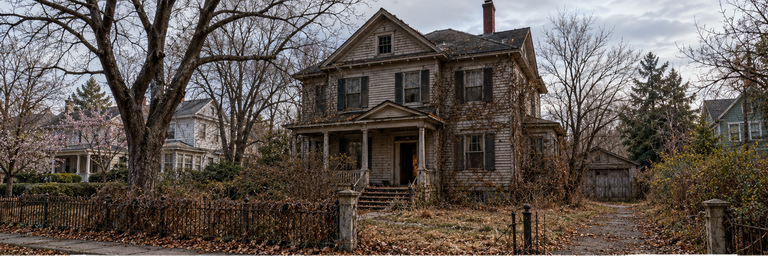
\includegraphics[width=\textwidth]{bilder/carlson-haus-aussen.png}
\caption{Während die Nachbarschaft den Frühling begrü\ss{}t, scheint das Carlson-Grundstück im Winter gefangen.}
\end{figure}
\begin{vorlesetextalle}
Die Adresse führt Euch in eine ruhige Wohnstra\ss{}e am Rande Arkhams. In den Gärten der Nachbarn zeigt sich bereits der Frühling: frische Knospen, saftiges Gras und hier und da das helle Wei\ss{} blühender Obstbäume. Kinderstimmen dringen aus der Ferne herüber, und über einem Zaun hängt frisch gewaschene Wäsche in der Sonne.

Doch das Grundstück, vor dem Ihr stehen bleibt, scheint einer anderen Jahreszeit anzugehören.

Das Haus der Carlsons ist ein gro\ss{}es, zweistöckiges Holzhaus der bürgerlichen Mittelschicht. Unter einem steilen, dunkel gedeckten Dach liegen zwei Reihen hoher Sprossenfenster. Eine überdachte Veranda zieht sich über die Vorderseite. Die einst hell gestrichenen Fassadenbretter sind grau und stumpf; tote Ranken umklammern das Geländer. Zwischen den Zaunlatten haben sich dürre Büsche und Unkraut ausgebreitet. Bis zum Haus führt ein Pfad, auf dem altes Laub in dicken Schichten liegt.

Es ist nicht der verwilderte Garten eines Winters. Es ist ein Grundstück, das aussieht, als sei es seit Jahrzehnten nicht mehr gepflegt worden. Ein paar Schritte weiter, hinter dem Nachbarzaun, blüht ein Strauch in voller Pracht. Hier aber rührt sich kaum ein Blatt.

Hinter den schmutzigen Fensterscheiben ist kein Licht zu erkennen. 
\end{vorlesetextalle}
\begin{meisterinfo}
\textbf{Verborgenes Erkennen (regulär):} Altes, mürbes Laub liegt auch an Stellen, die der Wind normalerweise freifegen würde; frische Triebe fehlen auffällig. Kein Wurf ist nötig, um den Kontrast zur Nachbarschaft zu bemerken. Eine höfliche Befragung der Nachbarn kann ergeben, dass zuletzt kaum jemand Helena gesehen hat; die Nachbarn können keine belastbare Erklärung liefern.
\end{meisterinfo}

\section{2.2 -- Die Veranda und die Stimme}
\begin{vorlesetextalle}
Die Verandadielen geben unter Euren Schritten ein leises, trockenes Knarren von sich. Auf den beiden Schaukelstühlen liegt eine graue Staubschicht. Ein umgekippter Blumentopf hat längst ausgedörrte Erde über die Bretter verteilt. Vor der Haustür sammeln sich verwitterte Blätter.

Die Haustür steht einen schmalen Spalt offen. Durch diesen seht Ihr einen dunklen Flur. Als Ihr klopft oder die Tür vorsichtig bewegt, hört Ihr aus dem Haus eine Frauenstimme:

\glqq{}Kommen Sie herein, ich bin gleich da! Sie können im Wohnzimmer Platz nehmen. Lassen Sie die Schuhe ruhig an.\grqq{}

Schritte entfernen sich in das Innere des Hauses. Dann herrscht wieder Stille.
\end{vorlesetextalle}
\begin{meisterinfo}
\textbf{Stimme:} Niemand erscheint. Wiederholtes Rufen bleibt unbeantwortet; keine zweite klare Ansage. Die Stimme klingt durchaus menschlich. Die Tür darf ohne Probe geöffnet werden. Die Ermittler können sich auch wieder zurückziehen und später zurückkehren.
\end{meisterinfo}

\section{2.3 -- Die Eingangsdiele}
\begin{vorlesetextalle}
Der Flur dahinter ist klein und kühl. Das wenige Tageslicht fällt durch trübe Scheiben auf einen dunkelblauen Teppich, dessen Muster fast im Grau verschwindet. Ein Garderobenschrank mit einigen Mänteln, ein Paar Lederstiefel und ein schmaler Konsolentisch stehen an den Wänden. Vertrocknete Blätter liegen überall auf dem Boden, vermischt mit Erde und Staub. Über einer kleinen Truhe hängt ein fleckiger Spiegel.

Die Luft riecht nach trockenem Holz, kalter Asche und altem Stoff. Seltsam ist die Temperatur: Obwohl drau\ss{}en die Frühlingssonne scheint, ist es hier kälter als im Schatten eines Kellers. Vor Euch führt eine Tür in einen grö\ss{}eren Raum.
\end{vorlesetextalle}
\begin{meisterinfo}
\textbf{Fund -- Brief 1 (17.10.1919):} Auf dem Konsolentisch liegt der erste Brief Flynns, halb unter einer Schale mit ausgetrockneten Blüten. \textbf{Verborgenes Erkennen:} Feine, erdige Abdrücke verlaufen über den Teppich; die Stiefel sind lange nicht getragen worden. Der Brief liegt auf einem etwas helleren, weniger verstaubten Fleck.
\end{meisterinfo}

\section{2.4 -- Der Wohnraum und die erste Vision}
\begin{figure}[htbp]\centering
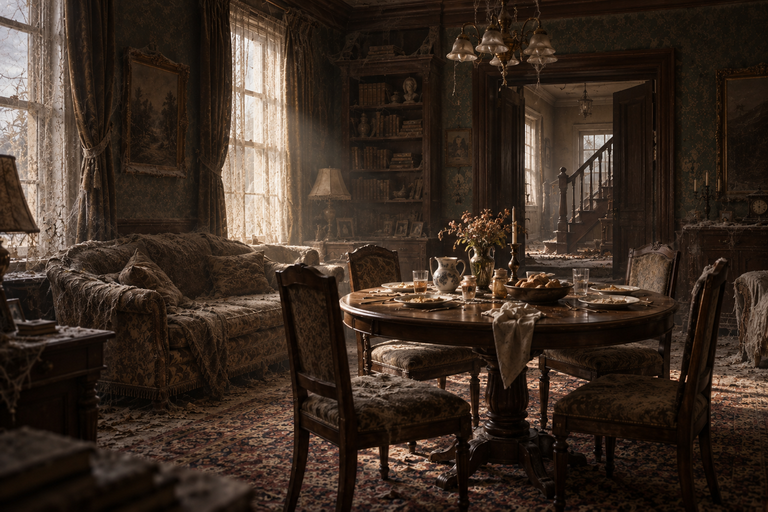
\includegraphics[width=\textwidth]{bilder/carlson-wohnzimmer.png}
\caption{Der Wohnraum: Staub auf Polstern und Möbeln, doch der runde Esstisch wirkt geradezu frisch benutzt.}
\end{figure}
\begin{vorlesetextalle}
Ihr betretet einen geräumigen Wohnraum. Ein Sofa, gepolsterte Sessel, ein Schrank mit Büchern und Porzellan, Bilderrahmen und dunkle Vorhänge zeugen von einer einst behaglichen Einrichtung. Alles ist unversehrt, aber wie unter einem grauen Schleier begraben. Staub liegt auf den Sitzpolstern, auf den Regalen, den Fensterbänken und dem Teppich. Spinnweben hängen an den Vorhangstangen. Man könnte glauben, seit Jahren habe niemand mehr dieses Zimmer betreten.

Nur der gro\ss{}e runde Esstisch in der Mitte widerspricht diesem Eindruck. Seine dunkle Platte ist frei von Staub. Auf ihr stehen Teller, Gläser und eine Karaffe, neben einer Serviette liegen Besteck und die Reste einer Mahlzeit. Es sieht aus, als sei jemand eben erst aufgestanden. Daneben liegen ein kleiner Messingschlüssel, ein ledergebundenes Buch und ein geöffneter Brief.

Eine weitere Tür führt zum hinteren Flur. Aus dieser Richtung dringt kein Laut. Die unnatürliche Stille lässt selbst die kleinsten Geräusche in Euren Ohren widerhallen.
\end{vorlesetextalle}
\begin{meisterinfo}
\textbf{Funde:} Brief 2 (21.10.1919) auf dem Tisch, Brief 3 (05.11.1919) hinter einer gerahmten Fotografie im Schrank. Der Messingschlüssel passt zur Kellertür. Das Lederbuch ist ein unverständlicher Auslöser der Vision; sein Inhalt ist hier nicht zu entziffern. \textbf{Verborgenes Erkennen:} Der Staub entspricht unmöglich nur einer Abwesenheit seit Herbst 1919. \textbf{Naturkunde / Spurensuche:} Feine, ungleichmä\ss{}ige Rillen am Türrahmen deuten nicht auf ein gewöhnliches Werkzeug hin.

\textbf{Auslöser:} Berühren oder bewusstes Untersuchen des Tisches, des Buchs oder der darauf liegenden Gegenstände. Alle Anwesenden werden Zeugen derselben Vision; der Auslöser braucht keine Probe.\end{meisterinfo}
\subsection{Vision I -- Der Verfolger}
\begin{vorlesetextalle}
Im Augenblick der Berührung wird Euch schwindlig. Das fahle Licht des Raumes kippt ins Warme; Staub und Spinnweben sind verschwunden. Ihr steht noch im selben Zimmer, doch die Luft riecht nach Essen und frischer Wäsche. Ihr könnt Euch bewegen, ohne einen Laut zu verursachen, als wärt Ihr blo\ss{}e Zuschauer.

Plötzlich fliegt die Tür zur Diele auf. Eine Frau in einem schlichten Kleid stürzt herein, die Hände an der Brust, den Blick voller Panik über die Schulter geworfen. Ihr Gesicht ist für einen Moment undeutlich wie hinter flie\ss{}endem Glas. Sie taumelt am Tisch vorbei und verschwindet durch die Tür zum hinteren Flur.

Ein Krachen erschüttert den Raum. Die Tür wird aus ihren Angeln gerissen, Holz splittert, und etwas Ungeheuerliches zwängt sich durch die Öffnung. Seine Gliedma\ss{}en sind viel zu lang, seine dunkle Gestalt zieht sich ruckartig zusammen und streckt sich wieder. Finger wie gebogene Klingen fahren über die Wand und rei\ss{}en tiefe Rillen in das Holz. Das Wesen folgt der Frau.

Mitten in der Bewegung hält es inne. Der schmale Kopf dreht sich langsam zurück. Es verharrt, als hätte es ein Geräusch gehört, das in dieser Zeit überhaupt nicht existieren dürfte.

Sein Blick richtet sich genau auf Euch.

Ein schriller, unmenschlicher Laut zerrei\ss{}t die Luft. Dann fällt alles in Dunkelheit. Als Ihr wieder sehen könnt, seid Ihr zurück im grauen Wohnraum. Der Tisch steht noch vor Euch. An der Wand und im Türrahmen zeichnen sich nun tiefe Kratzspuren ab.
\end{vorlesetextalle}
\begin{meisterinfo}
\textbf{Stabilität:} 1/1W4 STA. \textbf{Wichtig:} Das Wesen bemerkt die Beobachter \emph{scheinbar}, kann in der Vision aber nicht bekämpft werden. Die Ermittler werden nicht getrennt. Bei kreativen Versuchen einzugreifen bleibt der Kontakt zu den Gegenständen und zu Helena unwirklich. Die Kratzspuren sind nach der Vision eindeutig vorhanden.
\end{meisterinfo}

\subsection{Das Wesen in der Vision}
\begin{figure}[htbp]\centering
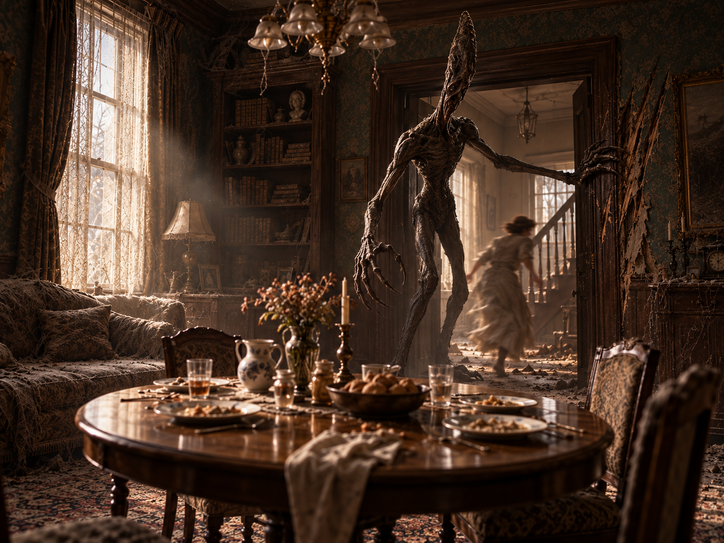
\includegraphics[width=0.95\textwidth]{bilder/gnicht-tyaacht-vision.png}
\caption{So könnte das Hrn-Tarl-Ya in der ersten Vision auf die Ermittler gewirkt haben.}
\end{figure}
\begin{meisterinfo}
\textbf{Erscheinungsbild:} Das Hrn-Tarl-Ya wirkt wie ein unnatürlich hochgewachsener, aus Holz, Haut und Schatten zusammengeflickter Verfolger. Seine Gliedma\ss{}en sind zu lang, die Bewegungen ruckartig und schnell, der Kopf schmal und fremdartig. Nutze die Illustration zur atmosphärischen Einordnung; die Spieler sollten das Wesen nicht lange und nie vollständig betrachten können.
\end{meisterinfo}

\section{2.5 -- Hinterer Flur und Treppenhaus}
\begin{vorlesetextalle}
Die zweite Tür führt in einen schmalen Flur. Eine Holztreppe steigt in das Obergeschoss hinauf, daneben liegt der Zugang zur Küche. Unter den Stufen befindet sich eine niedrige Tür. Über den Dielen liegt derselbe graue Film wie im übrigen Haus; ein verblasster Läufer ist an den Rändern steif geworden. An der Wand hängt schief ein Familienbild.

Auf dem Treppengeländer ziehen sich lange, unregelmä\ss{}ige Furchen nach oben. Ihr habt das Gefühl, dass sich die Kälte hier sammelt.
\end{vorlesetextalle}
\begin{meisterinfo}
Die Kellertür liegt unter der Treppe und ist verschlossen. Der Messingschlüssel aus dem Wohnzimmer öffnet sie. Andere Wege sind \emph{Schlosser} oder eine passende Kraftprobe; ein Fehlschlag kann Zeit oder Lärm kosten, darf die Erkundung aber nicht blockieren. Das Familienbild zeigt Flynn und Helena.
\end{meisterinfo}

\section{2.6 -- Die Küche}
\begin{vorlesetextalle}
In der Küche stehen ein gusseiserner Herd, eine Spüle und schwere Holzschränke. Auf einer Arbeitsplatte liegen ein Hackbrett und ein Messer; daneben stapelt sich ungewaschenes Geschirr. In einer Ecke ist ein kleiner Tisch teilweise mit einem verblichenen Tuch bedeckt. Eine umgesto\ss{}ene Schüssel hat vertrocknete Speisereste über die Dielen verteilt.

Auch hier ruht dicker Staub auf allem. An den Fenstern sitzt ein milchiger Beschlag, und der Atem scheint beim Sprechen fast sichtbar zu werden. In der Nähe des Herdes ist die vermeintliche Staubschicht nicht grau, sondern hell und kristallin.
\end{vorlesetextalle}
\begin{meisterinfo}
\textbf{Fund -- Brief 4 (22.11.1919):} In einer Schublade zwischen Tüchern. \textbf{Verborgenes Erkennen:} Was auf dem Herdrand wie Staub wirkt, ist feiner Reif. \textbf{Horchen:} Gelegentlich ein leises Kratzen, schwer zu orten, doch es scheint nicht aus den Wasserrohren zu stammen.
\end{meisterinfo}

\section{2.7 -- Der Keller}
\begin{vorlesetextalle}
Hinter der niedrigen Tür führt eine steile Holztreppe hinunter. Jeder Tritt gibt ein dumpfes Ächzen von sich. Die Luft wird schwer und erdig. Eine Laterne erhellt Kohlenvorräte, Regale mit Gläsern, Vorratskisten und einen alten Waschtrog.

In einer Ecke liegt eine Decke auf dem Boden. Daneben stehen ein fast leerer Wasserkrug und eine Petroleumlampe. Es sieht aus, als habe jemand sich hier versteckt. Innen an der Tür verlaufen mehrere tiefe, dicht beieinanderliegende Furchen. Die Holzsplitter zeigen in den Keller hinein.
\end{vorlesetextalle}
\begin{meisterinfo}
\textbf{Fund -- Brief 5 (17.12.1919):} In einer Blechdose unter der Decke. \textbf{Zusatzfund (optional):} Ein Zettel in Helenas Handschrift: \glqq{}Es kann Stimmen nachmachen. Ich höre es oben gehen.\grqq{} Diese Notiz ist \emph{neu} und gehört nicht zu den ursprünglichen Handouts. \textbf{Verborgenes Erkennen:} Ein Streifen lockerer Erde führt zu einer Ritze im Mauerwerk und endet dort ohne erkennbare Fortsetzung.
\end{meisterinfo}

\section{2.8 -- Gang im Obergeschoss}
\begin{vorlesetextalle}
Die Treppe mündet in einen schmalen, dunkleren Gang. Hier oben ist es noch kälter als unten. Durch die trüben Fenster fällt nur wenig Licht; an den Türgriffen hängt Staub wie eine zweite Patina. Drei Zimmertüren gehen vom Flur ab. Am Ende steigt eine schmale Holzstiege zu einer Luke unter dem Dach hinauf.
\end{vorlesetextalle}
\begin{meisterinfo}
Der Gang verbindet Schlafzimmer, Bad und früheres Gästezimmer beziehungsweise Lager. Wer länger lauscht, hört möglicherweise einmal trockenes Knacken über dem Kopf. Die Stiege zum Dachboden ist frei zugänglich.
\end{meisterinfo}

\section{2.9 -- Schlafzimmer}
\begin{vorlesetextalle}
Ein breites Bett mit sorgfältig gezogener Tagesdecke füllt den Raum. Zwei Nachttische, ein Kleiderschrank und eine Kommode stehen an den Wänden. Auf einer Spiegelablage liegen Bürste und Haarnadeln, daneben befindet sich ein gerahmtes Foto des Ehepaars. Flynns Kleidung hängt noch im Schrank, Helenas Kleider daneben.

Die Gegenstände erzählen von einem bewohnten Haus, das plötzlich verlassen wurde. Doch der Staub auf den Bettdecken scheint aus einer anderen Zeit zu stammen.
\end{vorlesetextalle}
\begin{meisterinfo}
\textbf{Fund -- Brief 6 (05.01.1920):} In der obersten Kommodenschublade. \textbf{Verborgenes Erkennen:} Kein Koffer fehlt, kein Reisekleid liegt bereit. Weitere Familienbilder sind vorhanden. Keine Probe ist nötig, um das Fehlen von Anzeichen einer geplanten Abreise zu erkennen.
\end{meisterinfo}

\section{2.10 -- Bad}
\begin{vorlesetextalle}
Das Bad ist klein, mit freistehender Wanne, Waschbecken und schmalem Spiegelschrank. Die Porzellanschalen sind stumpf, die Armaturen angelaufen. Auf dem Waschtisch stehen halb leere Fläschchen und eine Seifendose. Das Fenster ist von einem grauen Film überzogen. Ein Tropfen fällt irgendwo in das Waschbecken, doch die Leitung scheint trocken zu sein.
\end{vorlesetextalle}
\begin{meisterinfo}
\textbf{Fund -- Brief 7 (12.01.1920):} Gefaltet hinter den Fläschchen im Spiegelschrank. \textbf{Optionaler Gruseleffekt:} Ein Ermittler glaubt im Spiegel eine Gestalt hinter sich zu sehen; beim Umdrehen ist niemand dort. Keine Stabilitätsprobe, solange der Eindruck flüchtig bleibt.
\end{meisterinfo}

\section{2.11 -- Gäste- und Lagerzimmer}
\begin{vorlesetextalle}
Hier stehen unter fleckigen Leinentüchern kleine Möbel, ein alter Paravent, Hutschachteln und mehrere gestapelte Holzkisten. An einer Wand lehnt ein schmales Kinderbett ohne Matratze, offenbar lange nicht benutzt. Die Luft ist stickig, und bei jeder Bewegung wirbeln graue Flocken auf.
\end{vorlesetextalle}
\begin{meisterinfo}
\textbf{Fund -- Brief 8 (07.02.1920):} Zwischen alten Papieren in einer Hutschachtel. \textbf{Verborgenes Erkennen:} Eine Spur durch die Staubschicht läuft an der Wand entlang und endet abrupt über Bodenhöhe; sie ist mit menschlichen Schritten nicht leicht zu erklären.
\end{meisterinfo}

\section{2.12 -- Dachboden, letzter Brief und Bibliothekshinweis}
\begin{vorlesetextalle}
Die schmale Stiege endet unter einer Dachluke. Darüber liegt ein niedriger Dachboden, durchzogen von schweren Balken und unterbrochen von alten Truhen, Koffern und Möbelteilen. Ein kleines rundes Dachfenster lässt nur einen trüben Lichtfleck herein. Die Luft ist trocken und bei\ss{}end, und selbst das Knarren des Holzes scheint hier oben gedämpft.

An einem hohen Querbalken bewegt sich etwas kaum merklich im Luftzug. Zwischen zwei alten Kisten liegt eine schmale Mappe mit Papieren.
\end{vorlesetextalle}
\begin{meisterinfo}
\textbf{Funde:} Brief 9 (20.02.1920) in der Mappe; daneben der originale Handout-Zettel \glqq{}Archäologie in Ägypten von M. Dyers, 1899 -- Bücherei an der Miskatonic Universität -- EB8/II-474\grqq{}. Der Zettel führt unmittelbar zu Szene 3. \textbf{Verborgenes Erkennen:} Ein Seil verschwindet im Dämmerlicht über einem Balken; an ihm sind deutliche Scheuerstellen. Den Ermittlern darf die dunkle Gestalt zunächst entgehen, bis sie sich nähern oder mehr Licht schaffen.

\textbf{Räumliche Festlegung:} Die Erhängte befindet sich \emph{im Dachboden} unter dem Dach, nicht auf der gefährlichen Au\ss{}enseite des Dachs. Das entspricht der älteren Meisterskizze und erlaubt die geplante Lichtveränderung durch das Dachfenster.\end{meisterinfo}

\section{2.13 -- Helena Carlson: die zweite Vision}
\begin{vorlesetextalle}
Erst als Ihr Euch an die Schatten unter den Balken gewöhnt, erkennt Ihr, was dort hängt. Es ist eine Frau in einem schlichten Kleid. Ihr Körper schwebt reglos wenige Fingerbreit über den staubigen Dielen. Das Gesicht ist im Halbdunkel kaum zu erkennen, die Arme hängen schlaff herab.
\end{vorlesetextalle}
\begin{meisterinfo}
\textbf{Auslöser:} Berührung der Frau oder des Seils. Die Vision tritt für alle Anwesenden ein, die sich auf dem Dachboden befinden. Falls niemand die Gestalt berührt, kann das Licht bei einem vorsichtigen Untersuchungsversuch ebenfalls umschlagen. \textbf{Stabilität:} Beim Auffinden des Leichnams 0/1W3, bei der folgenden Vision 1/1W6 (Spielleiterentscheidung, kumulative Belastung beachten).
\end{meisterinfo}
\begin{vorlesetextalle}
In dem Augenblick, in dem Ihr den Körper berührt, verändert sich das Licht. Eben noch fiel nur ein trüber Schein durch das verschmutzte Dachfenster. Jetzt strömt helles Sonnenlicht herein, als wäre das Glas mit einem Schlag klar geworden. Die staubigen Balken leuchten goldbraun.

Die Frau hebt den Kopf. Ihre Augen sind geöffnet. Sie sieht Euch an, nicht mit blindem Schrecken, sondern mit einem schmerzlichen, dringlichen Blick. Langsam hebt sie ihren rechten Arm und streckt Euch die Hand entgegen.

\glqq{}Findet meinen Mann.\grqq{}

Ihre Lippen zittern.

\glqq{}Findet Flynn. Bitte ... rettet ihn.\grqq{}

Dann erlischt das Licht wie eine Kerze im Wind. Alles wird wieder grau. Das Seil schwingt leicht über Euch -- aber die Frau ist fort. Kein Körper liegt am Boden, kein Geräusch verrät, wohin sie verschwunden sein könnte.
\end{vorlesetextalle}

\section{2.14 -- Das Wesen im Haus}
\begin{vorlesetextalle}
Aus den unteren Stockwerken dringt ein Schrei, der nicht menschlich sein kann. Er beginnt tief und heiser, steigt in eine schneidende Höhe und bricht unvermittelt ab.

Danach hört Ihr Kratzen. Langsame, schwere Schläge gegen Holz, als würden lange Krallen an den Wänden entlangziehen. Das Geräusch bewegt sich unter Euch durch das Haus.

Wer vorsichtig durch die Dachbodenluke schaut, sieht im Halbdunkel des Ganges einen viel zu langen Arm, eine schmale Schulter und einen Kopf, der sich ruckartig bewegt. Dann verschwindet die Gestalt hinter der Treppenbiegung. Das Kratzen entfernt sich langsam.
\end{vorlesetextalle}
\begin{meisterinfo}
\textbf{Ziel:} Die Gefahr soll überwältigend wirken, aber keine zwangsläufige tödliche Falle darstellen. \textbf{Schleichen / Horchen:} Bei Gelingen erkennen die Ermittler eine günstige Pause und können sich leise zurückziehen. Bei einem Fehlschlag rückt das Kratzen näher oder eine Tür schlägt; es folgt nicht automatisch ein tödlicher Angriff. \textbf{Verhalten:} Warten, leise bleiben, dann gemeinsam das Haus verlassen. Wer aktiv gegen das Wesen vorgeht, erlebt seine erschreckende Überlegenheit; die konkreten Werte werden erst bei einer tatsächlichen Konfrontation benötigt.
\end{meisterinfo}

\subsection{Spielwerte des Hrn-Tarl-Ya}
\begin{figure}[htbp]\centering
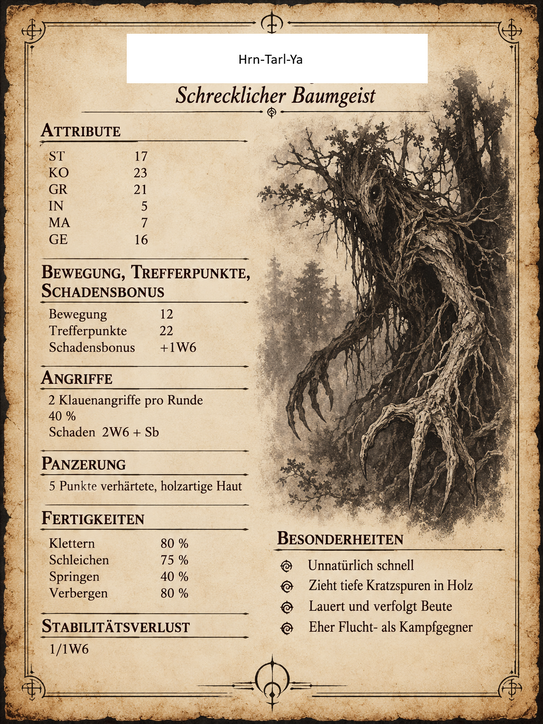
\includegraphics[width=0.82\textwidth]{bilder/gnicht-tyaacht-statblock.png}
\caption{Spielwerte des Hrn-Tarl-Ya für die Spielleitung.}
\end{figure}
\begin{meisterinfo}
\textbf{Einsatz im Abenteuer:} Diese Werte sind als Sicherheitsnetz für die Spielleitung gedacht. Das Wesen ist im Carlson-Haus in erster Linie ein Schrecken aus der Peripherie -- ein Verfolger, vor dem man flieht, nicht ein fairer Kampfgegner. Setze es sparsam ein: andeuten, hören lassen, kurz sehen lassen, Rückzug ermöglichen.

\textbf{Regelhinweis:} Der Stat-Block basiert auf Euren alten Unterlagen zum Hrn-Tarl-Ya und ist für die Szene leicht zugespitzt: zwei Klauenangriffe pro Runde, zähe holzartige Haut und hohe Werte in Schleichen, Klettern und Verbergen. Wenn Ihr die Szene rein erzählerisch halten wollt, reichen die Angaben im Flie\ss{}text bereits aus.
\end{meisterinfo}

\section{2.15 -- Flucht und Übergang zur Bibliothek}
\begin{vorlesetextalle}
Als Ihr endlich die Haustür hinter Euch lasst, weht Euch der warme Frühlingswind entgegen. In der Stra\ss{}e ist nichts verändert. Ein Vogel ruft, hinter dem Zaun des Nachbarn klappert Geschirr, und an einem Baum öffnen sich junge Blätter.

Das Haus der Carlsons steht grau und reglos hinter Euch. Sein Garten zeigt kein einziges Zeichen des Frühlings. Die Haustür bleibt einen schmalen Spalt offen.
\end{vorlesetextalle}
\begin{meisterinfo}
\textbf{Szenenergebnis:} Die Briefe dokumentieren Flynns Reise und den Zusammenbruch der Expedition. Helenas Vision bittet ausdrücklich darum, Flynn zu retten. Der Zettel mit dem Buchtitel und der Signatur führt die Gruppe in die Universitätsbibliothek. \textbf{Ausfallsicherung:} Werden Briefe übersehen, kann die Mappe auf dem Dachboden mehrere davon enthalten; der Bibliothekszettel sollte keinesfalls unauffindbar bleiben. \textbf{Nächste Szene:} Akt I, Szene 3 -- Das Geheimnis der Universitätsbibliothek.
\end{meisterinfo}

\chapter{Das Geheimnis der Universitätsbibliothek}
\noindent\textbf{Ort:} Bibliothek der Miskatonic University, Arkham\\
\textbf{Zeit:} Nach dem Besuch des Carlson-Hauses, voraussichtlich 5. April 1920\\
\textbf{Beteiligte:} Francis Collins, Lillie Johnson, Karim el-Mady, Natheniel Moss

\begin{meisterinfo}
\textbf{Szenenziel:} Den handschriftlichen Bibliothekszettel aus dem Dachboden aufgreifen; M. Dyers' Buch \emph{Archäologie in Ägypten} (1899) finden; die dort eingelegte Karte von Flynn Carlson mit dem Vermerk \emph{1920} untersuchen; einen versteckten Satz über die Grabkammern entziffern. Der Satz wird nicht nachträglich auf das vorhandene Karten-Handout geschrieben: Er ist lediglich als kaum sichtbare Druckspur auf dessen Papier gedacht.

\textbf{Wahrheit für die Spielleitung:} Flynn hat die Karte nicht selbst nach Arkham geschickt. Ihre Anwesenheit in diesem Buch ist eine erste, unaufgelöste Raum-Zeit-Anomalie im Zusammenhang mit dem sehenden Stein. Die Ermittler können das hier nicht beweisen. Auch Rudolf Greene kennt die Erklärung nicht. Die neue Hintergrundidee ist bewusst von den überlieferten Original-Handouts getrennt.

\textbf{Informationssicherung:} Das Buch, die Karte, die Signatur und das Haupt-Rätsel dürfen nicht durch einen misslungenen Einzelwurf verloren gehen. Misslungene Proben kosten Zeit, führen zu Teilinformationen oder machen Hilfe erforderlich.
\end{meisterinfo}

\section{3.1 -- Rückkehr zur Miskatonic University}
\begin{vorlesetextalle}
Das Licht des frühen Nachmittags liegt über den Wegen der Miskatonic University. Im Gegensatz zum Carlson-Haus scheinen hier die Bäume voller Leben zu sein: Knospen öffnen sich, Gespräche mischen sich mit dem Klacken eiliger Schritte, und irgendwo schlägt eine Uhr. Die vertraute Geschäftigkeit des Campus beruhigt Euch kaum. Was Ihr in jenem Haus gesehen habt, lässt sich nicht so leicht abschütteln.

Vor Euch erhebt sich das Bibliotheksgebäude, ein breiter Bau aus grauem Naturstein. Sein Eingang liegt hinter einer Reihe flacher Stufen; darüber stehen die Namen längst verstorbener Gelehrter in den Stein gemei\ss{}elt. Durch die hohen Fenster erkennt Ihr dunkle Regale und den warmen Schein elektrischer Lampen.
\end{vorlesetextalle}
\begin{meisterinfo}
Die Ermittler haben den Zettel \glqq{}Archäologie in Ägypten von M. Dyers, 1899 -- Bücherei an der Miskatonic Universität -- EB8/II-474\grqq{} aus dem Dachboden. Ohne diesen Zettel ist die gleiche Recherche über den Katalog möglich, braucht aber mehr Zeit.
\end{meisterinfo}

\section{3.2 -- Lesesaal und Auskunft}
\begin{vorlesetextalle}
Hinter der schweren Tür erwartet Euch eine hohe, stille Halle. Ein dunkler Holzfu\ss{}boden verschwindet unter langen Läufern. Reihen von Tischen mit grünen Leselampen stehen zwischen Säulen und hohen Regalen. Ledergebundene Bände füllen die Wände bis beinahe zur Decke; schmale eiserne Treppen führen auf eine Galerie. Es riecht nach Papier, Bohnerwachs und einem Hauch abgestandener Luft.

An einem Auskunftspult sortiert ein älterer Herr mit schmalem Gesicht und silbergrauem Haar Katalogkarten. Als Ihr näher tretet, legt er die Karten ordentlich zusammen und blickt über den Rand seiner Brille.
\end{vorlesetextalle}
\begin{meisterinfo}
\textbf{Rudolf Greene, Bibliothekar:} Ruhig, genau, etwas pedantisch. Er ist neugierig, sobald die Signatur genannt wird, aber keinesfalls eingeweiht. Die Figur stammt aus der älteren Arkham-Skizze. Er hilft der Gruppe, ohne neue Hintergrundgeheimnisse zu verraten.

\textbf{Möglicher Dialog:} \glqq{}Guten Tag. Haben Sie einen Titel oder eine Signatur für mich?\grqq{} -- Bei Vorlage des Zettels: \glqq{}EB8/II-474 ... einen Augenblick. Ägyptische Altertumskunde, ältere Bestände. Das sollte sich finden lassen.\grqq{}

\textbf{Bei Nachfragen zu Flynn:} \glqq{}An einen Herrn Carlson erinnere ich mich nicht sicher. Wir haben hier viele Wissenschaftler. Wenn das Buch hier liegt, dürfte es jedenfalls zur Sammlung gehören.\grqq{}

\textbf{Proben:} \emph{Bibliotheksnutzung} (regulär) ermöglicht selbstständiges Auffinden und die sichere Benutzung des alten Katalogs. Bei Fehlschlag bringt Greene das Buch nach einer kurzen Wartezeit. Eine Probe auf \emph{Charme}, \emph{Überreden} oder \emph{Psychologie} kann Gesprächsnuancen offenbaren, ist aber nicht erforderlich.
\end{meisterinfo}

\section{3.3 -- Das Buch von M. Dyers}
\begin{vorlesetextalle}
Wenig später liegt ein schwerer Band vor Euch. Sein dunkelgrüner Leineneinband ist an den Kanten abgesto\ss{}en, der goldgeprägte Titel nur noch teilweise zu erkennen: \emph{Archäologie in Ägypten}. Unter dem Verfassernamen M. Dyers steht das Erscheinungsjahr 1899.

Die Seiten enthalten Beschreibungen alter Ausgrabungen, Pläne, Zeichnungen von Reliefs und Fotografien in grobem Druck. Ein Kapitel berichtet von einer Expedition, die 1895 südlich von Luxor auf ungewöhnliche unterirdische Mauerzüge gesto\ss{}en sein soll. Zwischen den nüchternen wissenschaftlichen Abschnitten fallen einige vorsichtige Formulierungen auf: Die Bauweise lasse sich nicht recht einordnen; manche Steinarbeiten schienen älter als die umgebenden ägyptischen Anlagen.

An mehreren Stellen werden Statuen von schlanken, aufrecht stehenden Gestalten erwähnt. Die wenigen erhaltenen Skizzen zeigen glatte Gesichter und lange Gegenstände in ihren Händen, vielleicht Stäbe, vielleicht Waffen. Die Forscher gelangten offenbar nicht weit in die Anlage, bevor ihre Arbeiten abbrachen.
\end{vorlesetextalle}
\begin{meisterinfo}
\textbf{Hintergrund des Kapitels:} Dieser Grabungsbericht von 1895 ist ein neuer Baustein unseres Abenteuers. Er deutet die vorhandene Statuenhalle in der späteren Grabkammer an, ohne deren Funktion oder die Lösung vorwegzunehmen.

\textbf{Geschichte / Archäologie (regulär):} Die genannten Stilbrüche sind für eine ägyptische Grabanlage ungewöhnlich. \textbf{Schwieriger Erfolg:} Die Beschreibung klingt, als wäre eine ältere Struktur in späterer Zeit weiterverwendet worden. Bei Misserfolg fällt zumindest auf, dass die Autoren selbst keine überzeugende Datierung liefern.
\end{meisterinfo}

\section{3.4 -- Die eingelegte Karte}
\begin{vorlesetextalle}
Als Ihr die Seiten weiterblättert, lockert sich zwischen zwei Papierlagen ein gefaltetes Blatt und gleitet auf den Tisch. Es ist nicht mit dem Buch eingebunden, sondern offenbar irgendwann eingelegt worden.

Das Papier ist unregelmä\ss{}ig vergilbt und trägt eine handgezeichnete Karte: Gänge, Kammern, Abzweigungen, einzelne Zahlen und knappe Notizen. Die Linien wirken hastig, aber zielgerichtet. Einige Räume sind als leer bezeichnet, andernorts liegen besondere Fundorte oder blockierte Wege. Es ist keine Übersicht, wie man sie in einem gedruckten Lehrbuch erwarten würde.

Am Rand steht eine Signatur mit Datum: \emph{Flynn, 1920}.

Der Band in Euren Händen wurde 1899 veröffentlicht. Die Karte dagegen soll von jenem Mann stammen, der seit dem vergangenen Herbst in Ägypten verschollen ist. Wie gelangte seine Skizze ausgerechnet hierher?
\end{vorlesetextalle}
\begin{figure}[htbp]\centering
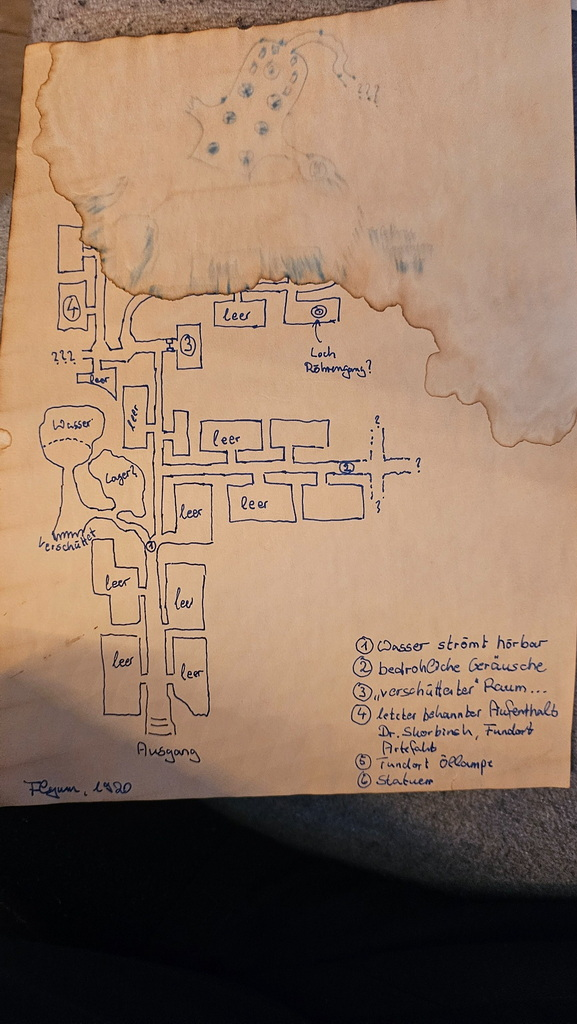
\includegraphics[width=0.85\textwidth,height=0.76\textheight,keepaspectratio]{bilder/flynn-grabkammerkarte-original.jpg}
\caption{Originales Karten-Handout: Flynns Skizze der unterirdischen Anlage (1920). Die sichtbaren Aufschriften bleiben unverändert.}
\end{figure}
\begin{meisterinfo}
\textbf{Ohne Probe:} Die Signatur \emph{Flynn, 1920} ist lesbar. Die Unstimmigkeit mit dem Erscheinungsjahr des Buches wird klar; sie ist noch kein Beweis für ein übernatürliches Ereignis, weil spätere Einlagen in Büchern grundsätzlich möglich sind.

\textbf{Bibliotheksnutzung (regulär):} In Ausleihunterlagen sind jüngere Vorgänge erkennbar, aber kein zuverlässiger Eintrag darüber, wann und von wem das lose Blatt eingelegt wurde. \textbf{Schwieriger Erfolg:} Die Aufzeichnungen liefern keinen nachvollziehbaren Weg der Karte von Ägypten nach Arkham. Es gibt keinen Nachweis, dass Flynn sie verschickt hätte. Greene kann ebenfalls keinen Absender nennen.

\textbf{Wichtig:} Die Karte selbst ist das vorhandene, fotografierte Original-Handout. Keine neue Legende, kein geänderter Text und keine räumliche Anpassung der Zeichnung wird vorausgesetzt.
\end{meisterinfo}

\section{3.5 -- Was das Papier bewahrt hat}
\begin{vorlesetextalle}
Beim längeren Betrachten fällt Euch auf, wie ungleichmä\ss{}ig das Papier gealtert ist. An einigen Stellen glänzt es flach, an anderen wirken die Linien vertieft. Zwischen den gezeichneten Kammern scheinen winzige Furchen zu liegen, die nicht zu den Wegen und Mauern gehören.
\end{vorlesetextalle}
\begin{meisterinfo}
\textbf{Untersuchung als gestufte Probe:}
\begin{itemize}
\item \textbf{Verborgenes Erkennen (regulär):} Die Ermittler entdecken zwischen den Kartenlinien blinde Druckspuren, die wie Schrift wirken. Ein schräg einfallender Lichtstrahl aus dem Fenster oder der Leselampe hebt sie hervor.
\item \textbf{Naturwissenschaft (Chemie), Handwerk oder eine geeignete fachliche Probe (regulär):} Durch vorsichtiges Beleuchten und Betrachten unter wechselnden Winkeln entziffern sie den verborgenen Satz. Eine chemische Behandlung ist \emph{nicht} erforderlich; eine Lupe kann helfen.
\item \textbf{Schwieriger Erfolg:} Die Druckspuren passen nicht zum Schriftbild der Kartenbeschriftungen, als sei der Satz auf einer anderen Unterlage entstanden und in die Karte eingedrückt worden.
\end{itemize}
\textbf{Ausfallsicherung:} Bei misslungenem Wurf erkennt ein aufmerksamer Charakter zumindest den Ansatz der Schrift; Rudolf Greene kann eine Leselampe mit beweglichem Schirm und eine Lupe bringen. Durch gemeinsames Probieren und etwas Zeit wird die Kernbotschaft sichtbar. Ein möglicher Preis ist Zeitverlust oder nur unvollständiges Verständnis, nicht der Verlust des Hinweises.
\end{meisterinfo}
\begin{vorlesetextalle}
Als Ihr das Blatt nun vorsichtig im schrägen Licht haltet, treten feine Vertiefungen hervor. Sie sind so schwach, dass Ihr zuerst nur einzelne Buchstaben wahrnehmt. Langsam formen sich Wörter, dann ein vollständiger Satz:

\begin{center}\itshape
\glqq{}Wir haben die Kammern nicht entdeckt. Man hat uns gestattet, sie zu betreten.\grqq{}
\end{center}

Darunter liegen weitere, nicht mehr lesbare Spuren. Einen Namen oder eine Erklärung findet Ihr nicht.
\end{vorlesetextalle}
\begin{meisterinfo}
\textbf{Deutung:} Der Satz deutet an, dass die Öffnung der Anlage kein Zufall war. Wer den Zutritt gewährte, bleibt unklar. Die Botschaft ist ein späterer Schlüssel zum Verständnis der Grabkammer, aber noch keine Anleitung, das Portal zu benutzen.

\textbf{Falls die Ermittler die Karte behalten wollen:} Greene erlaubt die Entnahme nicht einfach als regulären Bibliotheksvorgang. Er kann jedoch eine möglichst genaue Abschrift oder Abzeichnung ermöglichen; alternativ sind Überreden oder ein riskanter heimlicher Versuch denkbar. Für die weitere Expedition genügt eine gute Kopie der Karte.
\end{meisterinfo}

\section{3.6 -- Abschluss der Nachforschungen}
\begin{vorlesetextalle}
Als Ihr das Buch schlie\ss{}t, liegt das Kartenblatt noch immer auf dem Tisch. Drau\ss{}en ziehen die Schatten der Bäume über die hohen Fenster. In den Regalen raschelt eine Seite, und irgendwo wird ein Stuhl zurückgeschoben.

Ihr habt mehr gefunden, als Ihr erwartet hattet: einen Bericht über eine schwer einzuordnende Anlage südlich von Luxor, eine Karte von Flynn Carlson aus dem Jahr 1920 und eine Botschaft, die eher wie eine Warnung als wie eine wissenschaftliche Notiz klingt.

Aber die wichtigste Frage bleibt unbeantwortet: Wer hat Flynn und den anderen den Weg in die Tiefe geöffnet?
\end{vorlesetextalle}
\begin{meisterinfo}
\textbf{Ergebnis der Szene:} Die Gruppe kennt die archäologische Vorgeschichte, die spätere Rolle einer Statuenhalle wird vorbereitet, die Karte mit der Signatur \emph{Flynn, 1920} ist gefunden, und der rätselhafte Satz ist entschlüsselt. Die räumlich-zeitliche Unstimmigkeit wird nicht erklärt.

\textbf{Übergang:} Mit dem bibliothekarischen Hinweis endet die Ermittlungsphase in Arkham. Die Expedition nach Ägypten bleibt der nächste Schritt. Für Akt II sind Fahrpläne, Schiffsverbindungen, Reisedauer und das tatsächliche Ankunftsdatum noch historisch plausibel festzulegen.
\end{meisterinfo}


\chapter{Akt II -- Das Auge der Wüste}
\section{Szene 1 -- Aufbruch ins Ungewisse}
\begin{meisterinfo}
\textbf{Szenenziel.} Die Ermittler verlassen das vertraute Arkham, lernen den Alltag einer langen Reise von 1920 kennen und begegnen auf dem Atlantik Yusuf Hassan. Er ist ein vermisster Arbeiter aus Flynns Expedition, aber seine Erscheinung ist keine gewöhnliche Reisebekanntschaft. Die Szene soll neugierig machen, nicht den Mythos bereits erklären.

\textbf{Historischer Anker.} Die SS \emph{Adriatic} der White Star Line ist mit einer Abfahrt von New York nach Cherbourg und Southampton am \textbf{24. April 1920} in erhaltenen Passagierlisten belegt. Alle übrigen genauen Tage sowie die Anschlüsse in Europa sind eine \emph{plausible Szenario-Festlegung}, kein historisch belegter durchgehender Reiseplan. Alternativ kann die Spielleitung Schiff und Datum frei halten.

\textbf{Vorgeschlagene Chronologie:} 5. April Treffen mit Garmond; 6.--22. April Untersuchungen, Ausrüstung, Visa, Schiffsbuchung und Anreisevorbereitung; 23. April Bahn nach New York; 24. April Abfahrt der \emph{Adriatic}; Ende April/Anfang Mai Ankunft in Europa; Anfang Mai Bahn- und Kanalreise nach Marseille; darauf etwa fünf bis sieben Tage Mittelmeerfahrt mit einem passenden Passagierdampfer; um die zweite Maiwoche Alexandria und Weiterreise nach Kairo. Die genauen Anschlussdaten bleiben flexibel.

\textbf{Quellen zur historischen Einordnung:} GG Archives, \emph{White Star Line Passenger Lists 1889--1939}, Eintrag \emph{SS Adriatic, 24 April 1920}; \emph{Cairo of To-day}, Reisehinweise zur Seeverbindung Marseille--Alexandria (1897/98; Beleg der historischen Route, nicht eines Fahrplans für 1920).
\end{meisterinfo}

\subsection{1.1 -- Abschied von Arkham}
\begin{vorlesetextalle}
Die Tage nach Eurem Besuch in der Universitätsbibliothek vergehen zwischen Vorbereitungen, Briefwechseln und geschäftigen Besorgungen. Die Miskatonic University übernimmt die Kosten der Reise. Koffer werden gepackt, Unterlagen geordnet, dringend benötigte Ausrüstung beschafft. Zwischen den vielen kleinen Erledigungen bleibt immer wieder Zeit, an das Haus der Carlsons zurückzudenken: an den seltsam staubfreien Tisch, die Frau unter dem Dach und die Kreatur, die Euch aus einer Vergangenheit heraus anzusehen schien.

Als Ihr schlie\ss{}lich an einem kühlen Apriltag den Zug Richtung New York besteigt, liegt Arkham hinter Euch. Fabrikschornsteine, kleine Bahnhöfe und graue Vorstadtstra\ss{}en ziehen am Fenster vorbei. Vor Euch liegen ein Ozean, ein fremder Kontinent und die Suche nach Männern, deren letzte Nachrichten alles andere als beruhigend waren.
\end{vorlesetextalle}
\begin{meisterinfo}
\textbf{Spielraum:} Gib jeder Figur die Gelegenheit, eine persönliche Vorbereitung zu schildern. Nützliche Vorbereitungen sind Reisepapiere, Kleidung für die Wüste, Notizmaterial, Medikamente und eine sichere Aufbewahrung für Briefe und Karte. Gewöhnliche Ausrüstung soll nicht an Würfen scheitern. Eine \textbf{Bibliotheksnutzung}- oder \textbf{Wissen}-Probe darf Informationen zu den Verhältnissen in Ägypten liefern, aber keine zentrale Lösung vorwegnehmen.

\textbf{Kosten:} Gemä\ss{} Garmonds Auftrag finanziert die Universität Anreise, Passage und übliche Ausrüstung. Die Höhe etwaiger persönlicher Ausgaben ist für diese Szene nicht entscheidend.
\end{meisterinfo}

\subsection{1.2 -- Die Atlantiküberquerung}
\begin{vorlesetextalle}
New York empfängt Euch mit Lärm, Autohupen, den Rufen der Hafenarbeiter und dem unaufhörlichen Pfeifen der Dampfschiffe. Zwischen Kr\"anen und Lagerhäusern erhebt sich Euer Ozeandampfer: ein Schiff aus Stahl, mit hohen Schornsteinen, Rettungsbooten und Decks, die scheinbar nicht enden wollen.

Am 24. April verlasst Ihr den Hafen. Das Ufer fällt langsam zurück, bis die Stadt nur noch eine zackige Linie am Horizont ist. Die ersten Tage an Bord haben einen beinahe beruhigenden Rhythmus. Mahlzeiten werden zu festen Stunden serviert. Im Salon werden Zeitungen gelesen, an Deck promenieren Passagiere unter Decken und Mänteln, und das dumpfe Schlagen der Maschinen begleitet Euch bis in den Schlaf.

Im Lauf der Überfahrt verschwinden die letzten sichtbaren Spuren des Festlandes. Ringsum liegt nur der graublaue Atlantik. Selbst die Gespräche an Bord scheinen manchmal leiser zu werden, wenn die See besonders still ist.
\end{vorlesetextalle}
\begin{meisterinfo}
\textbf{Atmosphäre und Interaktion:} Kurze Gespräche mit anderen Reisenden, ein Rundgang über das Deck, eine Partie Karten oder ein Blick in die Schiffsbibliothek sind möglich. Erzähle einige Tage in geraffter Form; mache daraus keine zweite gro\ss{}e Ermittlungsphase. Auf dem Dampfer gibt es keine festgelegte Mythosbedrohung au\ss{}er der folgenden Begegnung.

\textbf{Ansto\ss{} zur Nebelszene:} Am sechsten Abend der Fahrt können die Ermittler nach dem Essen noch einmal auf das Promenadendeck gehen. Niemand muss eine Probe schaffen, um die Begegnung zu erleben. Falls alle in ihren Kabinen bleiben, bittet ein Steward um Hilfe bei einer offenstehenden Deckstür und lockt sie so nach drau\ss{}en, ohne die Situation zu erzwingen.
\end{meisterinfo}

\subsection{1.3 -- Der Fremde im Nebel}
\begin{vorlesetextalle}
Es ist die sechste Nacht Eurer Atlantiküberquerung. Seit dem Nachmittag liegt dichter Nebel über dem Meer. Anfangs waren es nur wei\ss{}e Schwaden gewesen, die über das Wasser zogen. Nun hat sich eine undurchdringliche graue Wand um das Schiff gelegt.

Das regelmä\ss{}ige Dröhnen der Maschinen reicht bis auf das Promenadendeck. In grö\ss{}eren Abständen ertönt das tiefe Nebelhorn. Der Klang verliert sich in der Dunkelheit, ohne ein Echo zurückzuwerfen.

Die meisten Passagiere haben sich längst in die Innenräume zurückgezogen. Die feuchten Decksplanken glänzen im Licht der vereinzelten Lampen. Am äu\ss{}eren Geländer steht ein Mann, den Ihr hier zuvor noch nicht bemerkt habt.

Er trägt einfache, abgetragene Kleidung und hat ein dunkles Tuch um seine Schultern geschlungen. Sein Rücken ist Euch zugewandt. Er starrt hinaus in den Nebel, als versuche er darin etwas zu erkennen.

Als Ihr näher kommt, dreht er langsam den Kopf. Sein Gesicht ist schmal und erschöpft, die Augen liegen tief in ihren Höhlen. Er mustert Euch einen Augenblick schweigend. Dann sagt er mit rauer, leiser Stimme:

\glqq{}Ihr sucht den Mann mit dem Stein.\grqq{}

Es klingt nicht wie eine Frage.

\glqq{}Er glaubt, er hätte etwas gefunden. Aber er hat etwas geöffnet.\grqq{}

Der Mann schaut hastig über die Schulter, als hätte jemand hinter ihm gesprochen.

\glqq{}Sagt Carlson, dass er den Augen nicht trauen darf.\grqq{}

Er tritt einen Schritt zurück. Der Nebel zieht in dichten Fäden zwischen Euch und das Geländer.

\glqq{}Mein Name ist Yusuf. Yusuf Hassan. Vergesst ihn nicht.\grqq{}

Ein langer Sto\ss{} des Nebelhorns fährt Euch durch Mark und Bein. Für einen Moment verschluckt der wirbelnde Nebel die Gestalt. Als Ihr wieder an dieselbe Stelle blickt, ist dort niemand mehr.
\end{vorlesetextalle}
\begin{meisterinfo}
\textbf{Wer ist Yusuf?} Yusuf Hassan ist ein ägyptischer Arbeiter aus der ursprünglichen Expedition. Flynn erwähnt in seinem Brief vom 7. Februar 1920 einen Arbeiter, der einem Schrei in die Anlage folgte und verschwand. \emph{Für unsere neue Fassung} erhält dieser bislang namenlose Mann den Namen Yusuf Hassan. Sein Tod ist nicht bestätigt.

\textbf{Spielweise:} Halte für Rückfragen einige knappe Sätze bereit. Auf \glqq{}Woher kennen Sie uns?\grqq{} erwidert er: \glqq{}Ich kenne nicht Euch. Aber der Stein schaut.\grqq{} Auf \glqq{}Wo ist Flynn?\grqq{} antwortet er: \glqq{}Hinter den Türen, die keine Türen sind.\grqq{} Bei Berührung ist sein Ärmel feucht und eiskalt. Die Begegnung endet, wenn sich der Nebel schlie\ss{}t oder ein Schiffssignal erklingt. Es gibt keine Verfolgungsjagd über die Reling; Yusuf verschwindet zwischen zwei Herzschlägen.

\textbf{Stabilität:} Noch keine Probe beim blo\ss{}en Gespräch. Der spätere Nachweis, dass Yusuf nicht an Bord war, rechtfertigt \textbf{0/1W3 STA}. Aufmerksame Ermittler können merken, dass er keine Schuhe trägt und trockene Sandkörner an den Fü\ss{}en haften. Diese Beobachtung erfordert \textbf{Verborgenes Erkennen (regulär)}, ist aber nicht nötig, um die Szene zu verstehen.
\end{meisterinfo}

\subsection{1.4 -- Ein Passagier, den es nicht gibt}
\begin{vorlesetextalle}
Einige Minuten später fährt das Schiff noch immer durch dichten Nebel. Ein Offizier der Nachtwache hört sich Euren Bericht mit zunehmendem Stirnrunzeln an. Er fragt nach Kleidung, Erscheinungsbild und Namen des Fremden.

\glqq{}Yusuf Hassan? Diesen Namen habe ich nie gehört. Warten Sie hier. Ich lasse nachsehen.\grqq{}

Nach einer Weile kehrt er mit einer Liste zurück. Er legt den Finger auf die eng beschriebenen Seiten und schüttelt langsam den Kopf.

\glqq{}Weder unter unseren Passagieren noch bei der Besatzung. Und ich versichere Ihnen: Während dieser Überfahrt ist niemand zugestiegen.\grqq{}
\end{vorlesetextalle}
\begin{meisterinfo}
\textbf{Nachforschungen:} Ein Gespräch mit dem Offizier und eine Prüfung des Verzeichnisses reichen aus, um Yusufs Abwesenheit zu bestätigen. \textbf{Überreden} oder \textbf{Charme} kann Zugang zum Originalverzeichnis verschaffen; auch ohne Erfolg wird die wesentliche Auskunft erteilt. \textbf{Verborgenes Erkennen (regulär)} an der Stelle der Begegnung entdeckt einige helle, ungewöhnlich trockene Sandkörner in den Fugen der nassen Planken. \textbf{Naturwissenschaft (Geologie)} kann vermuten, dass der feine Staub nicht typisch für eine salzige, feuchte Schiffsoberfläche ist; eine sichere geografische Herkunft lässt sich daraus nicht ableiten.

\textbf{Stabilität:} 0/1W3 STA, sobald die Ermittler begreifen, dass der Fremde dort nicht hätte sein können. Bei Fehlschlag auf soziale Proben wirkt der Offizier skeptischer, nicht unkooperativ. \textbf{Ausfallsicherung:} Wird der Name nicht notiert, lässt sich die Erinnerung später durch Aziz' Aussagen erneut auslösen.

\textbf{Spielleitergeheimnis:} Yusuf erscheint nicht als gewöhnlicher Geist. Er ist ein Echo, das durch die Störung von Raum und Zeit um den sehenden Stein entstanden ist. Damit wird auch die unmögliche Karte in der Bibliothek thematisch gespiegelt. Seine genaue Lage in den Katakomben bleibt für spätere Szenen offen; die Ermittler können ihn dort eventuell lebend, tot oder in einem Zwischenzustand finden. Das legen wir erst bei der Ausarbeitung der Grabkammer endgültig fest.
\end{meisterinfo}

\subsection{1.5 -- Über Europa}
\begin{vorlesetextalle}
Die letzten Tage auf dem Atlantik vergehen langsamer als zuvor. Immer wieder zieht es Euren Blick an jene Stelle des Decks, an der Yusuf gestanden hat. Doch weder im Licht der Morgensonne noch in weiteren Nebeln taucht er erneut auf.

Schlie\ss{}lich erscheint Land am Horizont. Europäische Hafenanlagen, Eisenbahnzüge, Zollbeamte und überfüllte Bahnsteige ersetzen die gleichförmige Weite des Ozeans. Ihr reist weiter Richtung Süden. Felder, Dörfer, Industriegebiete und gro\ss{}e Städte wechseln vor den Fenstern des Zuges, während sich mit jeder Etappe die Sprachen und die Gesichter um Euch verändern.

In Marseille liegt bereits das nächste Schiff vor Anker. Der salzige Geruch des Mittelmeeres, fremde Stimmen und die grelle Sonne über den Kais lassen die Atlantikreise wie einen weit entfernten Traum erscheinen.
\end{vorlesetextalle}
\begin{meisterinfo}
\textbf{Plausible Route:} Ankunft in Cherbourg beziehungsweise Southampton, dann Kanalquerung und Eisenbahnreise über Frankreich nach Marseille. Die konkrete Zugfolge und die Mittelmeerabfahrt sind bewusst nicht als historisch belegte April-/Mai-1920-Fahrpläne ausgegeben. Falls die Gruppe Europastopps ausspielen möchte, eignet sich eine kurze Begegnung mit einem Zollbeamten oder Reisevertreter, jedoch ohne neues Rätsel.
\end{meisterinfo}

\subsection{1.6 -- Das Mittelmeer und die Küste Ägyptens}
\begin{vorlesetextalle}
Das Mittelmeer zeigt sich Euch in einem anderen Licht. Das Wasser liegt heller und blauer unter einem beinahe makellosen Himmel. In der Ferne ziehen Frachter und Segelschiffe vorbei, über den Decks kreisen Möwen. Die Abende sind milder, die Luft riecht nach Salz und Maschinenöl.

Nach weiteren Tagen auf See erscheint schlie\ss{}lich die flache Küste Ägyptens. Zuerst sind nur helle Linien im Dunst zu erkennen, dann Kräne, Masten und die Häuser Alexandrias. Zwischen Rufen, Gepäckwagen und Zollformalitäten betretet Ihr zum ersten Mal ägyptischen Boden.

Die letzte Etappe führt mit der Eisenbahn nach Kairo. Durch das Fenster ziehen Felder, Dörfer und Wasserläufe vorbei. Hier und da öffnen sich Blicke auf eine Landschaft, deren Farben Ihr aus keinem Neuengland-Frühling kennt.

Als der Zug in den Bahnhof von Kairo einrollt, ist aus der Reise ein neues Kapitel geworden. Vor Euch liegt die Stadt, in der Flynn Carlson und Dr. Skorbinsk ihre Unternehmung begonnen haben.
\end{vorlesetextalle}
\begin{meisterinfo}
\textbf{Anschluss:} Akt II, Szene 2 -- \emph{Kairo, das Tor zum Orient}. Die Ermittler suchen zunächst das Hotel International auf. Dort soll der Kontakt zu Aziz wiederhergestellt werden.

\textbf{Spätere Rückbindung:} Wenn die Gruppe Aziz den Namen Yusuf Hassan nennt, erkennt er ihn als einen der vermissten Arbeiter wieder. Besonders wirkungsvoll ist ein altes Mannschaftsfoto, auf dem Yusuf zu sehen ist. Foto und Aussehen müssen erst in der Kairo-Szene festgelegt werden; hier ist noch kein zusätzliches Handout nötig.

\textbf{Leitmotiv:} Von der Karte \glqq{}Flynn, 1920\grqq{} über die Visionen im Carlson-Haus bis zu Yusufs Erscheinung auf See häufen sich Hinweise darauf, dass Orte und Zeiten rund um die Grabkammer nicht zuverlässig voneinander getrennt sind. Die Ursache wird in dieser Szene nicht erklärt.
\end{meisterinfo}

\chapter{Kairo -- Das Tor zum Orient}
\noindent\textbf{Ort:} Kairo, Ägypten; Hotel International und Stadtgebiet\\
\textbf{Zeit:} Mai 1920, nach der Reise von Arkham\\
\textbf{Beteiligte:} Francis Collins, Lillie Johnson, Karim el-Mady, Natheniel Moss; Aziz

\begin{meisterinfo}
\textbf{Szenenziel:} Kairo als lebendige Stadt vorstellen, den verlässlichen Übersetzer und Organisator Aziz etablieren, die Ereignisse um Yusuf Hassan rückwirkend verstörend machen und die Reise nach Luxor und zur Ausgrabungsstätte vorbereiten. Aziz ist herzlich, kräftig, lebensfroh und mutig -- und hat eine feste Grenze: Er begleitet die Gruppe bis zum Lager, nicht in die unterirdischen Kammern. Kein einzelner misslungener Wurf darf den Aufbruch verhindern.

\textbf{Kontinuität:} Flynn Carlson und Dr.~Skorbinsk wohnten im Oktober 1919 im Hotel International. Aziz half bei Expedition und Übersetzungen und übernahm Flynns letzten Brief an Helena. Yusuf Hassan ist der verschollene Arbeiter, dem die Ermittler vermeintlich auf dem Atlantik begegneten. Die Zeitphänomene und Zeichen sind noch nicht vollständig erklärt.
\end{meisterinfo}

\section{2.1 -- Ankunft in Kairo}
\begin{figure}[htbp]\centering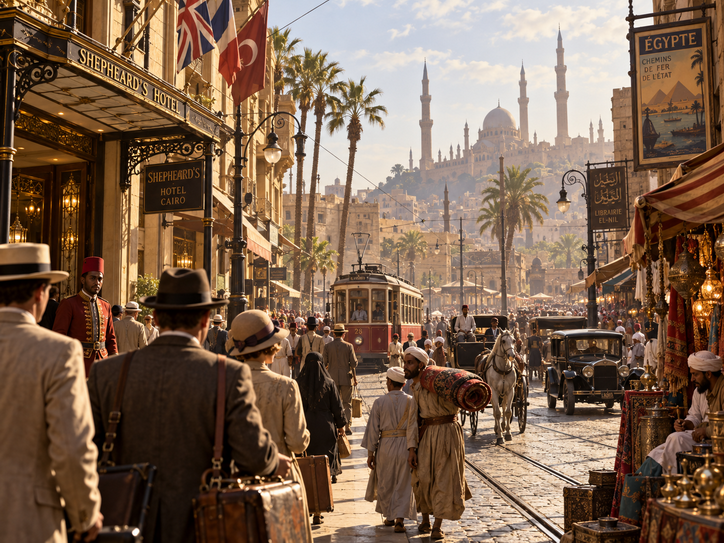
\includegraphics[width=\textwidth]{bilder/kairo-strassenszene.png}\caption{Kairo: Stra\ss{}enbahnen, Wagen, Hotelviertel und das geschäftige Stadtleben. Atmosphärische Illustration, keine historische Fotografie.}\end{figure}
\begin{vorlesetextalle}
Nach der langen Reise erreicht Ihr endlich Kairo. Schon im Bahnhofsgebäude schlägt Euch warme, trockene Luft entgegen. Gepäckträger rufen einander zu, Koffer poltern über Steinplatten, aus vielen Richtungen hört Ihr Gespräche in verschiedenen Sprachen. Unter dem hohen Dach mischen sich die Pfeifsignale der Eisenbahn mit dem Rattern von Handwagen.

Drau\ss{}en erwartet Euch eine Stadt in stetiger Bewegung. Eine Stra\ss{}enbahn rumpelt um die Ecke, ein Automobil hupt hinter einem von Pferden gezogenen Wagen. Händler preisen ihre Waren an, Zeitungsjungen rufen Schlagzeilen, und Menschen in Anzügen, Kleidern, langen Gewändern und unterschiedlichen Kopfbedeckungen drängen sich zwischen Cafés und Geschäften. Über den Dächern zeichnen sich Kuppeln und Minarette ab. Warmer Staub, Gewürze, Tabakrauch und der Duft frisch gebackenen Brotes liegen in der Luft.

Nach Wochen des Reisens erscheint Euch alles gleichzeitig fremd und von beinahe überwältigender Lebendigkeit. Ihr seid in Ägypten angekommen.
\end{vorlesetextalle}
\begin{meisterinfo}
\textbf{Freies Spiel:} Die Gruppe kann Gepäck organisieren, nach dem Hotel fragen, Geld wechseln, den Stra\ss{}enverkehr beobachten oder ein Fahrzeug nehmen. Karim el-Mady kann seine Sprachkenntnisse sinnvoll einsetzen; Ortskenntnis ist damit nicht automatisch gegeben. Keine Pflichtproben. Wer mit Anwohnern spricht, begegnet unterschiedlichen Auffassungen über die politische Lage und ausländische Ausgrabungen, ohne dass daraus ein zusätzlicher Handlungsstrang entstehen muss.
\end{meisterinfo}

\section{2.2 -- Das Hotel International}
\begin{vorlesetextalle}
Euer Wagen hält vor einem stattlichen Hotel mit heller Fassade und breitem Vordach. Gepäckträger eilen herbei. Durch hohe Glastüren gelangt Ihr in eine kühle, gro\ss{}zügige Halle mit Steinboden, dunklen Holzverkleidungen und Messingleuchten. Gro\ss{}e Topfpflanzen flankieren den Empfang. Hoch über Euch bewegen sich Deckenventilatoren träge durch die warme Luft.

Hinter dem Tresen werden Gästebücher aufgeschlagen, Zimmerkarten gereicht und Koffer auf kleine Wagen geladen. Aus einem Salon dringen gedämpftes Stimmengewirr und das Klirren von Teegläsern. Nach den vielen Reisetagen wirkt dieser Ort beinahe unwirklich komfortabel.
\end{vorlesetextalle}
\begin{meisterinfo}
Die Miskatonic University hat Zimmer reserviert. Das Hotel ist ein fiktiver beziehungsweise abenteuerinterner Schauplatz; die Illustration der Stra\ss{}enszene zeigt ein anderes reales Hotel und dient nur der Atmosphäre. Eine Nachfrage beim Empfang bestätigt die Aufenthalte von Flynn Carlson und Dr.~Skorbinsk im Oktober 1919. \textbf{Bibliotheksnutzung (im Register) oder Überreden/Charme (beim Personal):} Ein Angestellter erinnert sich an Skorbinsks häufige Besuche und seine ungehaltenen Nachfragen nach Post; Flynn wirkte freundlicher, aber zuletzt angespannt. Diese Informationen sind fakultativ und dürfen auch ohne Probe durch höfliches Nachfragen zugänglich sein.
\end{meisterinfo}

\section{2.3 -- Aziz stellt sich vor}
\begin{figure}[htbp]\centering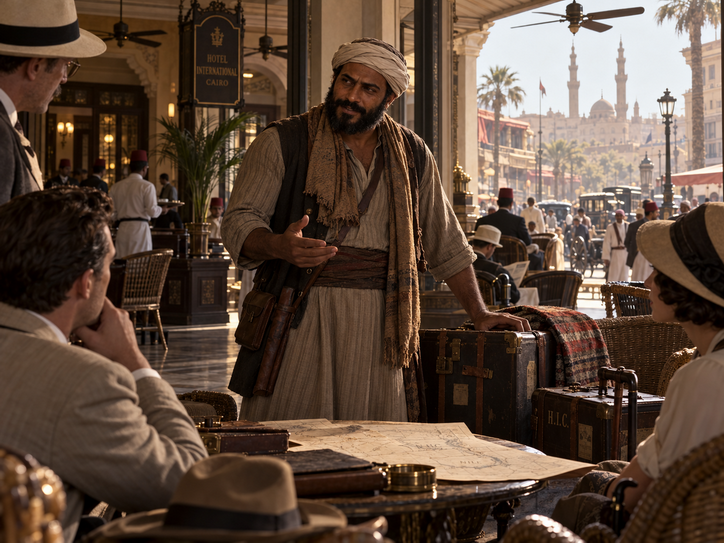
\includegraphics[width=\textwidth]{bilder/aziz-hotel-international.png}\caption{Aziz begrü\ss{}t die Ermittler im Hotel International -- ein kräftiger, humorvoller Mann mit Lebenserfahrung.}\end{figure}
\begin{vorlesetextalle}
Im Salon habt Ihr gerade Platz genommen, als ein kräftiger, breitschultriger Mann mit dichtem dunklem Bart und sonnengebräuntem Gesicht auf Euch zukommt. Seine Kleidung ist zweckmä\ss{}ig, seine Umhängetasche sichtbar viel benutzt. Ausgeprägte Lachfalten umrahmen die Augen, die Euch wach und neugierig mustern.

Der Mann breitet die Arme aus, als begrü\ss{}e er alte Freunde. 

\glqq{}Meine Freunde! Ihr müsst die Herrschaften von der Miskatonic University sein!\grqq{}

Er lacht, reicht Euch nacheinander die Hand und stellt sich vor: \glqq{}Aziz. Einfach Aziz! Ich habe mit Euren Professoren gearbeitet. Mit Carlson und mit diesem anderen Herrn ... Skorbinsk! Bei Allah, dieser Mann konnte einen zur Verzweiflung bringen!\grqq{}

Er winkt einem Kellner. \glqq{}Tee für uns! Und etwas zu essen. Meine neuen Freunde sehen aus, als hätten sie eine lange Reise hinter sich.\grqq{} Dann setzt er sich mit einem zufriedenen Seufzen. \glqq{}Nun erzählt: Was führt Euch in unser schönes Kairo? Doch wohl nicht nur die Aussicht auf guten Tee?\grqq{}
\end{vorlesetextalle}
\begin{meisterinfo}
\textbf{Aziz (etwa 40):} Kräftig, bärtig, lebensfroh, handfest, laut lachend, ortskundig, erfahren in Übersetzung und Reiseorganisation. Er nimmt die Gruppe ernst und behandelt sie zunächst als Gäste. Er ist kein eingeschüchterter Überlebender und kein heimlicher Gegner. Er scherzt über Dr.~Skorbinsks Verschlossenheit, respektiert Flynn und hält nichts davon, Warnzeichen zu ignorieren. Er erklärt von sich aus, dass er die Expedition bis zum Lager begleitet hatte und zuletzt mit Flynns Brief abreiste.

\textbf{Psychologie (regulär):} Beim Thema Katakomben wird Aziz ernst, nicht ängstlich: Er wägt seine Worte ab, weil er die Gefahr nicht leichtfertig kleinreden möchte. Bei Fehlschlag ist die Veränderung seines Tons dennoch bemerkbar.
\end{meisterinfo}
\subsection{Das Gespräch über die Ausgrabung}
\noindent\textbf{Aziz auf Fragen nach dem Ort:}
\begin{quote}\glqq{}Hört zu, meine Freunde. Ich habe Sandstürme erlebt, die ganze Karawanen verschlucken können, und Männer getroffen, die gefährlicher sind als Schlangen. Aber dort unter den Felsen stimmt etwas nicht. Ich wei\ss{} nicht, was es ist. Und ich will es auch gar nicht wissen. Ein vernünftiger Mann hört auf seinen Verstand.\grqq{}\end{quote}
\noindent\textbf{Aziz über die Wissenschaftler:}
\begin{quote}\glqq{}Carlson wollte Antworten. Skorbinsk glaubte schon, sie zu besitzen. Das ist ein gro\ss{}er Unterschied.\grqq{}\end{quote}
\begin{meisterinfo}
Aziz berichtet ohne Probe: Arbeiter verlie\ss{}en den Ort, in der Anlage ertönten unerklärliche Geräusche, Skorbinsk wurde zunehmend verschlossen, Flynn blieb zurück. Er kennt die Anlage nicht vollständig und behauptet nicht, das Rätsel lösen zu können. Auf konkrete Fragen nach dem sehenden Stein berichtet er nur von Skorbinsks Fixierung auf einen Gegenstand; dessen Funktion kennt er nicht.
\end{meisterinfo}

\subsection{Yusuf Hassan -- die Erinnerung an das Schiff}
\noindent\textbf{Falls die Ermittler Yusuf erwähnen:}
\begin{quote}\glqq{}Yusuf Hassan? Ja, ich kannte Yusuf. Ein guter Junge, flei\ss{}ig und immer zu Scherzen aufgelegt. Er ging in die unteren Kammern und kam nicht wieder zurück. Wir haben gesucht. Niemand hat ihn seitdem gesehen.\grqq{}\end{quote}
\noindent\textbf{Nach dem Bericht über die Begegnung im Nebel:}
\begin{quote}\glqq{}Nein, das kann nicht sein. Yusuf war nicht auf Eurem Schiff.\grqq{}\end{quote}
\begin{meisterinfo}
Aziz wird still und mustert die Gruppe, ohne in Panik zu geraten. Dann: \glqq{}Vielleicht solltet Ihr mir genauer erzählen, was Ihr gesehen habt.\grqq{} Ein gelungenes \textbf{Überreden, Charme oder Psychologie} kann zu einer genaueren Beschreibung Yusufs und der Umstände seines Verschwindens führen. Falls die Gruppe nicht von Yusuf berichtet, bleibt dieser Gesprächsteil aus; der Zusammenhang kann später am Lager wieder aufgegriffen werden. Ein Foto der Expeditionsmannschaft wäre ein mögliches späteres Handout, ist derzeit jedoch nicht Bestandteil der vorhandenen Materialien.
\end{meisterinfo}

\section{2.4 -- Aziz' Bedingungen}
\begin{vorlesetextalle}
Aziz stellt sein Teeglas ab und legt die breiten Hände auf den Tisch.

\glqq{}Also gut, meine Freunde. Ich bringe Euch nach Luxor. Ich besorge die Wagen, die Leute und alles, was Ihr braucht. Wenn Ihr darauf besteht, führe ich Euch bis zum Lager.\grqq{}

Er hebt einen Finger. \glqq{}Aber dort ist Schluss. Ich werde keinen einzigen Schritt in diese verfluchten Gänge setzen. Versteht mich nicht falsch: Ich bin kein Feigling. Aber es gibt einen Unterschied zwischen Mut und Dummheit.\grqq{}

Ein warmes, entschlossenes Lächeln kehrt auf sein Gesicht zurück.

\glqq{}Ihr wollt Carlson finden? Dann helfe ich Euch. Doch mit den Dingen, die dort unten geschehen, will ich nichts zu tun haben.\grqq{}
\end{vorlesetextalle}
\begin{meisterinfo}
\textbf{Spielmechanik:} Aziz' Begleitung bis zum Lager steht fest; eine Probe auf Überreden oder Charme ist dafür nicht notwendig. Gute Argumente und gelungene soziale Proben können ihm zusätzliche Erklärungen, Kontakte, eine Reserveausrüstung oder einige weitere Tage Logistik am Lager entlocken. \textbf{Unverrückbar:} Er betritt weder die Grabkammer noch die Katakomben. Das ist eine begründete Entscheidung eines erfahrenen Mannes, keine Feigheit. \textbf{Falls die Gruppe ihn bedrängt:} Er bleibt freundlich, wird aber bestimmt: \glqq{}Meine Antwort bleibt nein.\grqq{}
\end{meisterinfo}

\section{2.5 -- Das Zeichen an der Zimmertür}
\begin{vorlesetextalle}
Spät am Abend ist das Hotel ruhig geworden. Von der Stra\ss{}e dringt nur noch ein gedämpftes Rauschen herauf. Dann hört Ihr drei langsame Schläge gegen Holz.

Als Ihr die Zimmertür öffnet, ist der Gang leer. Die Wandlampen werfen gelbliche Lichtinseln auf den Boden. Unmittelbar vor der Schwelle liegt eine feine Spur Sand. Sie führt ein paar Schritte weit und endet ohne erkennbare Fortsetzung.

Auf der Innenseite der Tür seht Ihr etwas, das Euch zuvor nicht aufgefallen ist: ein in das Holz eingeritztes Zeichen, ein Oval mit einem Punkt darin und einem gebogenen Fortsatz darunter. Ihr kennt dieses Symbol bereits.
\end{vorlesetextalle}
\begin{meisterinfo}
\textbf{Verborgenes Erkennen oder passende Handwerksfertigkeit (regulär):} Die Kerben sind dunkel und wirken erstaunlich alt, nicht frisch eingeschnitten. Der Sand ist feinkörnig und trocken. Weitere Recherchen bei der Nachtschicht führen zu keinem beobachteten Besucher. Am Morgen ist das Zeichen verschwunden; die Tür ist glatt, und auch die Sandspur fehlt. \textbf{Stabilität:} 0/1W3 STA, sobald die Ermittler die Unmöglichkeit des Vorfalls begreifen. \textbf{Inszenierung:} Kein weiteres Gespenst, keine Verfolgung. Die kurze Störung setzt das wiederkehrende Motiv von gestörtem Raum und Zeit fort und sollte nicht vorzeitig erklärt werden.
\end{meisterinfo}

\section{2.6 -- Die Vorbereitungen für die Wüste}
\begin{figure}[htbp]\centering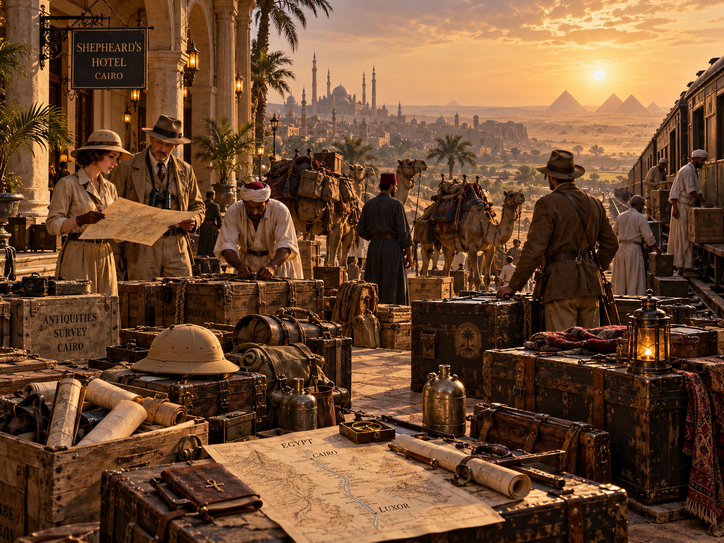
\includegraphics[width=\textwidth]{bilder/kairo-expeditionsvorbereitung.png}\caption{Vorbereitungen für den Aufbruch nach Luxor: Proviant, Werkzeug, Karten und Transportmittel. Atmosphärische Illustration.}\end{figure}
\begin{vorlesetextalle}
Am nächsten Morgen herrscht geschäftiges Treiben. Aziz steht zwischen Koffern, Holzkisten und aufgerollten Decken, prüft Lieferlisten und gibt mit lauter Stimme Anweisungen. Zwischendurch scherzt er mit den Trägern, klopft einem Fuhrmann auf die Schulter und überprüft selbst den Verschluss einer Wasserkiste.

Als er Euch bemerkt, lacht er. \glqq{}Gut! Ihr seid also wach. Ich kümmere mich um die Reise. Ihr kümmert Euch darum, nicht allzu viel unnötigen Unsinn einzupacken. In der Wüste werdet Ihr jedes überflüssige Pfund verfluchen!\grqq{}

Er zeigt auf Karten, Proviant und Ausrüstung, die in sorgfältigen Reihen bereitliegen. \glqq{}Jetzt esst erst einmal ordentlich. Wer wei\ss{}, wann Ihr wieder eine anständige Mahlzeit bekommt!\grqq{}
\end{vorlesetextalle}
\begin{meisterinfo}
\textbf{Grundausstattung:} Aziz organisiert Wasserbehälter und Reservewasser, haltbaren Proviant, Zelte, Decken, Petroleum- oder Öllampen samt Brennstoff, Seile, Werkzeuge und geeignete Transportmöglichkeiten. Er empfiehlt zudem Sonnenschutz, festes Schuhwerk und eine kleine medizinische Ausrüstung. Die Gruppe kann selbst zusätzliche Dinge beschaffen (etwa Fotografieausrüstung, Messgeräte, Skizzenmaterial, weitere Lampen). \textbf{Eigene Entscheidungen:} Sinnvolle Sonderwünsche dürfen Kosten oder Zeit verlangen, sollen aber nicht die Haupthandlung blockieren.

\textbf{Reiseplan:} Zunächst geht es nach Luxor; von dort führt Aziz die Ermittler weiter zum Lager. Die Distanz und der genaue Zeitbedarf dieser letzten Etappe werden mit der nächsten Szene festgelegt. \textbf{Übergang:} Szene 3 -- Das verlassene Expeditionslager.
\end{meisterinfo}


\chapter{Das verlassene Expeditionslager}
\noindent\textbf{Akt II -- Szene 3.} Letzte Etappe von Luxor zum Fundort; Abschied von Aziz; freie Erkundung des Lagers.
\begin{meisterinfo}
\textbf{Überblick:} Hier gibt es keine lebenden Expeditionsmitglieder und keine Leichen. Die Ermittler sollen den Ort als überstürzt verlassen erleben, sich mit Material ausrüsten und die Vorgeschichte von Flynn Carlson, Dr. Skorbinsk und Yusuf Hassan vertiefen. Die zuvor gefundene Karte bleibt das zentrale Navigationsmittel im folgenden Dungeon. Aziz ist lebensfroh, kräftig und verlässlich; er betritt die unterirdischen Kammern jedoch unter keinen Umständen. Die vier Zonen des Lagers können in beliebiger Reihenfolge untersucht werden.

\textbf{Zeit:} Später Nachmittag, nach der Reise aus Luxor. Richtzeiten für die Reise bitte als Abenteuerchronologie behandeln, nicht als dokumentierte Fahrpläne.
\end{meisterinfo}
\section{3.1 -- Die letzten Meilen}
\begin{figure}[htbp]\centering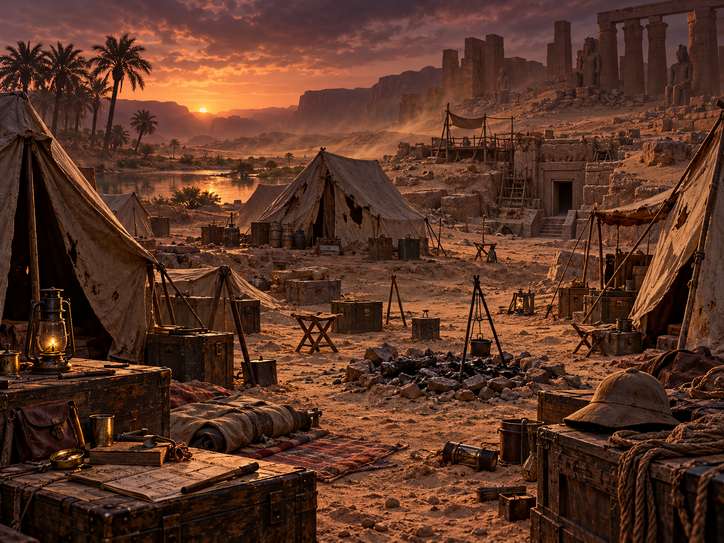
\includegraphics[width=\textwidth]{bilder/lager-verlassen.png}\caption{Das verlassen wirkende Expeditionslager in der ägyptischen Felslandschaft.}\end{figure}
\begin{vorlesetextalle}
Seit dem frühen Morgen seid Ihr unterwegs. Die grünen Felder am Nil liegen weit hinter Euch. Gelbbraune Hügel und ausgedörrte Felsen haben die Landschaft übernommen. Die Sonne steht unerbittlich über den Wagen; selbst das Leder Eures Gepäcks scheint hei\ss{} geworden zu sein. Wenn ein Rad gegen einen Stein schlägt, hallt das Geräusch zwischen den Felswänden wider.

Aziz hat die Fahrt mit Liedern und Geschichten begleitet und sich scherzhaft über die Qualität des Weges beklagt. Doch als der Tross eine niedrige Anhöhe erreicht, verstummt er. Vor Euch liegt eine von Felswänden eingefasste Senke. Ihr erkennt Zelte, verstreute Kisten, aufragende Gestelle und eine dunkle Öffnung im Fels. Kein Mensch bewegt sich zwischen den Zelten.

Aziz hält an. Er mustert die Szene und sagt leise: \glqq{}Da wären wir. Das ist Carlsons Lager. Aber jemand sollte hier sein. Wenigstens die Wächter. Oder der Koch.\grqq{}
\end{vorlesetextalle}
\begin{meisterinfo}
\textbf{Verborgenes Erkennen:} Einige Zelte stehen noch, andere sind eingefallen; Werkzeuge liegen achtlos herum. \textbf{Spurensuche:} Verwaschene Wagen- und Fu\ss{}spuren, aber kein nachvollziehbarer geordneter Abzug. \textbf{Geologie:} An einzelnen Felswänden sind frische Spalten zu erkennen. Kein Wurf ist erforderlich, um das vollständige Fehlen der Menschen zu erkennen.
\end{meisterinfo}
\section{3.2 -- Aziz zieht seine Grenze}
\begin{vorlesetextalle}
Aziz steigt vom Wagen, verschränkt die Arme vor seiner breiten Brust und betrachtet die stillen Zelte. \glqq{}Was für ein Empfang! Nicht einmal jemand, der uns Tee anbietet.\grqq{} Er schmunzelt, aber diesmal klingt das Lachen kürzer als sonst.

\glqq{}Als ich zuletzt hier war, wurde gehämmert, gestritten und gekocht. Jetzt hört man nicht einmal einen Esel. Ich helfe Euch beim Lager, bei der Ausrüstung, bei allem, was ein vernünftiger Mensch tun kann.\grqq{}

Er deutet auf den dunklen Eingang in der Felswand. \glqq{}Aber dort unten hört meine Hilfe auf. Das habe ich Euch versprochen, und ich halte Wort. Ich bin kein Feigling. Ich wei\ss{} nur, wann Mut in Dummheit umschlägt.\grqq{}
\end{vorlesetextalle}
\begin{meisterinfo}
Aziz hilft bei Vorräten, Lampen, Seilen und der Lagererkundung. Er bietet an, bis zum nächsten Morgen zu warten oder später zu einem vereinbarten Termin zurückzukehren. Er lässt sich auch durch beste \emph{Überreden}-Würfe nicht zum Betreten der Grabkammer bewegen. \textbf{Psychologie:} Er ist entschlossen und besorgt, aber nicht panisch. \textbf{Bei Nachfragen:} In der Tiefe hörte er Stimmen vermeintlich längst verschwundener Arbeiter. Aziz darf Kenntnisse über den Weg zum Lager oder dessen Organisation beisteuern; er kennt die jüngsten Ereignisse in den Katakomben nicht.
\end{meisterinfo}
\section{3.3 -- Zwischen Zelten und Kisten}
\begin{vorlesetextalle}
Zwischen den Zelten rascheln lose Planen im Wind. Auf einer Pritsche liegt eine zerknitterte Decke; daneben stehen Stiefel, als sei ihr Besitzer kurz hinausgegangen. Eine Feuerstelle ist erloschen. Im Topf hängen eingetrocknete Essensreste. Schaufeln, Seile und Instrumentenkisten sind liegengelassen worden. Ein Stuhl liegt umgestürzt, eine Tasse steht halb im Sand.

Das Lager sieht nicht ordentlich aufgegeben aus. Es ist, als hätten seine Bewohner ihre Arbeit mitten in einem gewöhnlichen Tag unterbrochen und seien einfach nicht zurückgekommen.
\end{vorlesetextalle}
\subsection{A -- Das Arbeitszelt Flynns}
\begin{vorlesetextalle}
Unter einem ausgeblichenen Zeltdach steht ein Arbeitstisch voller Vermessungsblätter, Bleistifte und Skizzen. Über einer Kiste hängt eine Jacke. Ein Feldstuhl liegt auf der Seite. Die letzte Seite eines offen liegenden Notizhefts ist mit hastiger Schrift gefüllt.
\end{vorlesetextalle}
\begin{meisterinfo}
\textbf{Bibliotheksnutzung oder Verborgenes Erkennen:} Zwischen den Notizen lässt sich ein Eintrag entziffern: \glqq{}Ich habe die Gänge gestern vermessen. Heute stimmen die Entfernungen nicht mehr. Entweder unterlaufen mir Fehler, oder die Anlage verändert sich.\grqq{} Wer die Karte aus Arkham mitbringt, kann Flynns Wegmarken mit den eigenen Beobachtungen vergleichen. Der Eintrag ist auch ohne Probe bei gründlicher Durchsicht zugänglich.
\end{meisterinfo}
\subsection{B -- Das Zelt Dr. Skorbinsks}
\begin{vorlesetextalle}
Bücherkisten, wissenschaftliche Instrumente und unordentliche Blätterstapel füllen das Zelt. Auf mehreren Seiten kehrt dasselbe seltsame Augensymbol wieder. Neben einer Lupe liegen verschmierte Zeichnungen eines handtellergro\ss{}en Steins.
\end{vorlesetextalle}
\begin{meisterinfo}
\textbf{Archäologie:} Viele der Zeichen passen nicht zu bekannter ägyptischer Schrift. \textbf{Okkultismus:} Skorbinsk scheint denselben Gegenstand aus widersprüchlichen Blickrichtungen beschrieben zu haben. \textbf{Aufzeichnungen:} Der Doktor behandelte das Artefakt zunehmend als sein ausschlie\ss{}liches Forschungsobjekt. Seine Person oder das Artefakt selbst befinden sich nicht im Zelt.
\end{meisterinfo}
\subsection{C -- Mannschaftszelte und Kochstelle}
\begin{vorlesetextalle}
Hier stehen einfache Feldbetten und Bündel mit persönlichen Dingen. Auf einer Plane liegen eine Bürste, eine Schale, grobe Arbeitskleidung und eine kleine Stofftasche. Das Feuer ist längst kalt.
\end{vorlesetextalle}
\begin{meisterinfo}
\textbf{Schlüsselbefund:} In der Tasche steht der Name \emph{Yusuf Hassan}. Darin liegen ein Kamm und ein kleiner Messinganhänger mit einer eingravierten Blüte. Ein Gruppenfoto zeigt Yusuf unter Arbeitern der Expedition: die Ermittler erkennen den Mann von der Atlantiküberfahrt. Keine Probe darf diese Wiedererkennung verhindern, falls die Spieler nach Yusuf suchen. \textbf{Psychologie:} Die wenigen zurückgelassenen Habseligkeiten sprechen gegen einen geplanten Aufbruch.
\end{meisterinfo}
\subsection{D -- Das Materiallager}
\begin{vorlesetextalle}
Holzkisten stehen unter einer halb gelösten Plane. Ihr findet Ersatzdochte, Lampenöl, Schaufeln, Hacken, Seile, leere Wasserkanister und ein beschädigtes Vermessungsgerät. Ein Teil des Materials ist brauchbar; anderes hat unter dem Sand gelitten.
\end{vorlesetextalle}
\begin{meisterinfo}
\textbf{Vorbereitung:} Genügend Seile, Wasser, Lampen und einfaches Werkzeug sind verfügbar. \textbf{Mechanische Reparaturen:} Eine defekte Lampe oder ein Vermessungsinstrument kann instand gesetzt werden. \textbf{Spielerinitiative belohnen:} Mehrere Lichtquellen, ein Sicherungsseil und eine markierte Rückroute helfen später bei Sandfalle, Orientierung und Flucht vor dem Dhole. Ressourcen dürfen hier frei geplant werden.
\end{meisterinfo}
\section{3.4 -- Eine Nacht voller Geräusche}
\begin{vorlesetextalle}
Die Sonne ist hinter den Felsen verschwunden. Der Himmel ist schwarz und voller Sterne. Das Feuer knistert, und bei jeder Böe schlagen die Zeltseile gegen ihre Pfosten. Dann dringt aus der Richtung des Eingangs ein dumpfes Rollen, gefolgt von einem tiefen, schleifenden Laut. Unter Euren Fü\ss{}en scheint der Boden kurz zu zittern. Alles wird wieder still.
\end{vorlesetextalle}
\begin{meisterinfo}
\textbf{Horchen oder Geologie:} Die Geräusche erinnern an Bewegungen unter der Erde, sind aber nicht sicher als gewöhnlicher Felssturz erklärbar. Aziz sieht die Ermittler nur ernst an: \glqq{}Ja. Genau das meine ich.\grqq{} Keine erneute Vision. Ein Nachtlager, eine Wache oder ein sofortiger Aufbruch bleiben freie Entscheidungen. \textbf{Abschied:} Aziz verabschiedet sich am Eingang mit kräftigem Händedruck: \glqq{}Wenn Ihr Stimmen hört, ruft nicht gleich zurück. Und kommt wieder heraus, meine Freunde.\grqq{}
\end{meisterinfo}


\chapter{Die Kammern der Vergessenen}
\noindent\textbf{Akt II -- Szene 4.} Offener Dungeon-Crawl bis unmittelbar vor die Statuenhalle.
\begin{meisterinfo}
\textbf{Grundprinzip:} Die Gruppe besitzt Flynns handgezeichnete Karte von 1920 und die Briefe an Helena sowie die Informationen aus M. Dyers' Buch. Die Karte bleibt gültige Grundlage der Navigation, auch wenn einige Gänge in der Wirklichkeit von der Zeichnung abweichen. Kleine leere Räume können zusammenfassend erzählt werden. Die wesentlichen Stationen -- verschüttete Kammer, Öllampe, Yusuf, Wasserstelle, Dhole, Wächterleichname und Statuenportal -- lassen sich über die Karte und die Spuren frei ansteuern. Hindernisse sind keine Einbahnstra\ss{}e; kreative Lösungen ermöglichen Alternativen. \textbf{Fortsetzung:} Die vier Statuen und das bereits geöffnete Dimensionstor erscheinen erst im folgenden Kapitel.
\end{meisterinfo}
\section{4.1 -- Der Eingang in die Tiefe}
\begin{figure}[htbp]\centering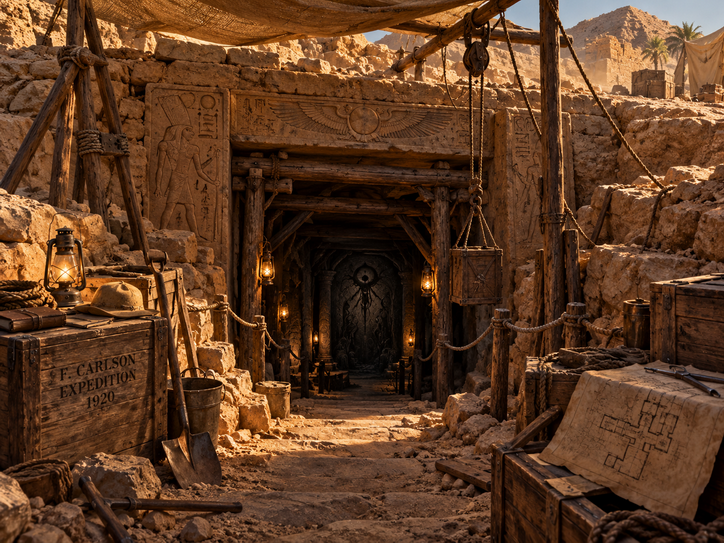
\includegraphics[width=\textwidth]{bilder/eingang-grabkammer.png}\caption{Der von der Expedition erschlossene Zugang zu den unterirdischen Kammern.}\end{figure}
\begin{vorlesetextalle}
Am Fu\ss{} einer niedrigen Felswand sichern hölzerne Stützen eine aus dem Gestein geschlagene Öffnung. Seile und eine einfache Winde hängen neben Werkzeugkisten. Eine schmale Treppe führt hinunter in das Dunkel. Mit jedem Schritt wird die Luft kühler. Das Licht Eurer Lampen tastet über Steinblöcke, verblasste Reliefs und geometrische Linien im Fels. Einige Bearbeitungsspuren sind neu, andere scheinen aus unvorstellbar ferner Zeit zu stammen. Hinter Euch schrumpft die helle Öffnung des Eingangs.
\end{vorlesetextalle}
\begin{meisterinfo}
\textbf{Archäologie:} Die Grundanlage passt nicht zu einer üblichen ägyptischen Grabanlage; manche Motive scheinen später ergänzt. \textbf{Verborgenes Erkennen:} Moderne Markierungen der Ausgräber. \textbf{Orientierung:} Bei Verwendung der Karte ist eine grundsätzliche Positionsbestimmung ohne ständigen Wurf möglich. \textbf{Horchen:} Tief unten scheint Wasser zu flie\ss{}en.
\end{meisterinfo}
\section{4.2 -- Die leeren Räume}
\begin{vorlesetextalle}
Kammer folgt auf Kammer. Manche besitzen Nischen, andere niedrige Sockel, doch alles ist leer. Auf den Böden liegt feiner Staub, in den vereinzelt die Schuhabdrücke der Expedition eingedrückt sind. Wiederholt führen breite Gänge in schmale Abzweigungen. Ihr habt das Gefühl, dass die Entfernung zwischen den Räumen auf Eurer Karte kürzer ausfällt als die Wege, die Ihr tatsächlich zurücklegt.
\end{vorlesetextalle}
\begin{meisterinfo}
\textbf{Interaktion:} Markierungen mit Kreide, Schnur oder Wegskizzen vereinfachen die Rückkehr. \textbf{Verborgenes Erkennen:} Spuren von verschobenen Steinblöcken und abgebrochene Werkzeugteile. \textbf{Archäologie:} Es fehlen typische Bestattungsmerkmale; die Anlage wirkt eher wie ein System aus Übergängen. \textbf{Keine Sackgasse:} Auch ein misslungener Orientierungswurf erzeugt Verzug, keine willkürliche Trennung der Gruppe.
\end{meisterinfo}
\section{4.3 -- Die verschüttete Kammer}
\begin{vorlesetextalle}
Ein breiter Raum ist teilweise unter einer gewaltigen Menge Sand und Geröll verschwunden. Zwischen den Massen ragen zerbrochene Stützbalken hervor; auf einem Block liegt eine Schaufel. Ein Seilende verschwindet unter dem Sand. Doch die Decke über Euch ist makellos. Nirgends zeigt sich die Bruchstelle, aus der diese Massen hätten stammen können.
\end{vorlesetextalle}
\begin{meisterinfo}
\textbf{Wiedererkennung:} Flynns Brief vom Januar berichtete von einem verschütteten Arbeiter und einer später plötzlich wieder intakten Kammer. \textbf{Geologie:} Der Sand passt mengenmä\ss{}ig nicht zum Raum. \textbf{Verborgenes Erkennen:} Ein Stück Arbeitskleidung ragt aus dem Sand. \textbf{Ausgraben:} Mit Seilen und Werkzeugen lassen sich sterbliche Überreste des Arbeiters freilegen (0/1W3 STA). Der Fund ist optional; der Raum bleibt auch ohne Freilegung bedeutend.
\end{meisterinfo}
\subsection{Die Sandfalle}
\begin{vorlesetextalle}
Ein leises Rieseln ertönt über Euren Köpfen. Zwischen den Steinplatten quillt Sand hervor. Ein dünner Strahl wird zu einer stiebenden Kaskade. Aus mehreren Wandnischen ergie\ss{}t sich trockenes Material auf den Boden. Es wird mehr -- viel mehr, als irgendwo hinter den Wänden Platz finden dürfte. Innerhalb weniger Augenblicke bedeckt Sand Eure Schuhe und steigt weiter.
\end{vorlesetextalle}
\begin{meisterinfo}
\textbf{Vier Gefahrenstufen:} (1) Knöchel, (2) Knie, (3) Hüfte, (4) Raum fast gefüllt. Nach jeder gewichtigen Handlung steigt die Stufe; clevere Hilfsmittel verzögern den Anstieg. \textbf{Lösungen:} Klettern über Nischen, Stärke zum Herausziehen, Seile als Sicherung, Mechanische Reparaturen zur Stabilisierung einer Tür, Verborgenes Erkennen für eine erhöhte Öffnung, gemeinsame Flucht über den bekannten Eingang. Misslungene Proben kosten Zeit oder Ausrüstung. Kein unvorbereiteter sofortiger Tod. \textbf{Nachwirkung:} Bei späterer Rückkehr kann der Raum vollkommen leer und unversehrt sein (1/1W4 STA). Der Widerspruch zu Flynns Briefen soll klar werden.
\end{meisterinfo}
\section{4.4 -- Dr. Skorbinsks Öllampe}
\begin{vorlesetextalle}
In einer unregelmä\ss{}igen Kammer liegen verschobene Platten und Scherben. Eine Petroleumlampe steht aufrecht mitten im Raum, als hätte jemand sie soeben dort abgestellt. Neben ihr liegen Kreide, ein beschädigtes Notizheft und ein einzelner Handschuh. Auf der Steinplatte daneben sind hastige Linien zu einem Kreis mit vier Markierungen eingeritzt.
\end{vorlesetextalle}
\begin{meisterinfo}
\textbf{Fund:} Die Lampe ist die von Flynn erwähnte Öllampe Dr. Skorbinsks. Das Heft enthält Bruchstücke: \glqq{}Der Stein reagiert nicht auf Licht. Er reagiert auf den Blick.\grqq{} / \glqq{}Die vier Wächter sind keine Abbilder. Sie bewachen etwas.\grqq{} / \glqq{}Ich glaube zu verstehen, warum die Kammern leer sind.\grqq{} \textbf{Verborgenes Erkennen:} Die vier Markierungen sind symmetrisch. \textbf{Archäologie:} Keine übliche Grabanordnung. \textbf{Okkultismus:} Vielleicht Ritual oder Mechanismus. \textbf{Mechanische Reparaturen:} Lampe reparierbar. Kein Körper des Doktors.
\end{meisterinfo}
\subsection{Der Fund des sehenden Steins}
\begin{vorlesetextalle}
Hinter einer halb verschobenen Steinplatte erkennt Ihr eine flache, sorgfältig aus dem Fels gemei\ss{}elte Nische. Darin liegt ein handtellergro\ss{}er, grauer Stein. Sein Umriss ist unregelma\ss{}ig und seine Oberfläche glatt geschliffen. Auf einer Seite befindet sich ein eigentümliches Zeichen: ein stilisiertes Auge aus einer ovalen Linie, einem Punkt und einem geschwungenen Fortsatz. Dieses Symbol kennt Ihr aus den Briefen und den Aufzeichnungen der Expedition.
\end{vorlesetextalle}
\begin{meisterinfo}
\textbf{Verbindlicher Fund:} Dies ist der \emph{sehende Stein}, das in Flynns Brief vom 5. Januar 1920 beschriebene Artefakt. Er liegt in einer Nische einer angrenzenden Kammer unweit von Skorbinsks Öllampe. Flynn berichtet am 20. Februar, den Stein erneut gefunden zu haben; nachdem er in die andere Dimension geriet, blieb er hier zurück. \textbf{Kein Wurf nötig:} Wer den Raum absucht, entdeckt die Nische und nimmt den Stein mit. \textbf{Verborgenes Erkennen:} Die umliegende Staubspur deutet auf eine erst kürzlich bewegte Platte. \textbf{Archäologie/Okkultismus:} Das Zeichen entspricht keiner eindeutig zuordenbaren ägyptischen Schrift; der Stein scheint in eine eigens dafür gearbeitete Fassung zu gehören. \textbf{Ausfallsicherung:} Wird diese Kammer ausgelassen, finden die Ermittler den Stein deutlich sichtbar unmittelbar vor dem offenen Tor in der Statuenhalle. Er ist stets zugänglich; das Finale hängt nicht von einem verdeckten Suchwurf ab. \textbf{Besitz:} Notiere, wer den Stein mitnimmt; er bleibt bis zum Einsetzen in die Plattform in dieser Person Besitz.
\end{meisterinfo}

\section{4.5 -- Die Spur von Yusuf Hassan}
\begin{vorlesetextalle}
Der Gang verengt sich an einer Kreuzung. Auf dem Boden liegt eine zerbrochene Laterne, daneben eine dunkle, eingetrocknete Spur. Jemand hat Buchstaben in die Wand gekratzt. Sie sind ungelenk und enden abrupt: \textbf{YUSUF}. Darunter findet Ihr weitere, deutlich schwächere Schriftzeichen.
\end{vorlesetextalle}
\begin{meisterinfo}
\textbf{Arabisch:} Karim el-Mady kann bei entsprechender Sprachkenntnis ohne Probe übersetzen: \glqq{}Es sieht durch uns.\grqq{} Andere Charaktere benötigen eine passende Sprachprobe oder Hilfe. \textbf{Verborgenes Erkennen:} Ein schmaler Messinganhänger mit einer eingeritzten Blüte liegt in einer Ritze. Er ähnelt dem Fund in Yusufs Tasche -- derselbe Mann erschien auf dem Atlantik. \textbf{Wahrheit für die Spielleitung:} Yusuf ist in der Anlage verschollen. Die Erscheinung an Bord war kein gewöhnlicher Geist, sondern ein räumlich-zeitliches Echo. Nicht behaupten, sein Tod sei sicher belegt; die alten Briefe berichten nur von seinem Verschwinden. \textbf{Stabilität:} Nach Erkennen der unmöglichen Verbindung optional 0/1W3.
\end{meisterinfo}
\section{4.6 -- Die unterirdische Wasserstelle}
\begin{vorlesetextalle}
Ein leises Flie\ss{}en wird zu deutlichem Rauschen. Der behauene Gang öffnet sich in eine natürliche Höhle. Feuchter Stein glänzt im Lampenlicht. Wasser sickert aus einer Felsöffnung und verschwindet unter einer niedrigen Steinbrücke. Hier unten ist die Luft überraschend kühl. In der spiegelnden Oberfläche laufen plötzlich breite Wellen auseinander, obwohl niemand das Wasser berührt hat. Von fern kommt ein tiefes, vibrierendes Grollen.
\end{vorlesetextalle}
\begin{meisterinfo}
\textbf{Geologie:} Älteres natürliches Höhlensystem; \textbf{Horchen:} Das Grollen ist nicht durch Wasser allein erklärbar. \textbf{Verborgenes Erkennen:} Breite Schleifspuren an den Wänden. \textbf{Vorbereitung:} Ein niedriger Seitenraum nahe der Wasserstelle eignet sich als Versteck. Er kann bereits vor der Dhole-Begegnung entdeckt und markiert werden.
\end{meisterinfo}
\section{4.7 -- Der Dhole}
\begin{figure}[htbp]\centering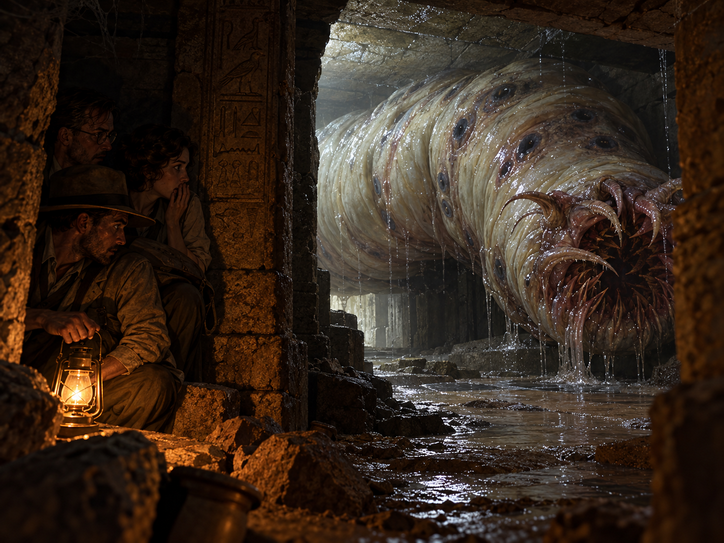
\includegraphics[width=\textwidth]{bilder/dhole.png}\caption{Der ungeheure Dhole ist eine Flucht- und Versteckbegegnung, kein gewöhnlicher Kampf.}\end{figure}
\begin{vorlesetextalle}
Ein dumpfer Schlag erschüttert den Boden, dann ein zweiter, näherer. Staub rieselt von der Decke. Ein tiefes Grollen geht in ein feuchtes, schmatzendes Schaben über. Hinter der nächsten Biegung drängt sich bleiche Masse in den Gang, viel zu gro\ss{} für jeden natürlichen Bewohner dieser Höhlen. In ihrer Oberfläche öffnen sich dunkle Vertiefungen. Vorn klafft ein ungeheures, von gebogenen Zähnen umgebenes Maul. Das Wesen schiebt sich weiter auf Euch zu und füllt fast den gesamten Gang.
\end{vorlesetextalle}
\begin{meisterinfo}
\textbf{Stabilität:} 1W4/1W10 STA (dramatischer Szenenrichtwert). \textbf{Fluchtphase:} Orientierung mit Flynns Karte zeigt einen Seitenraum; Verborgenes Erkennen entdeckt eine nahe Spalte; Klettern, Stärke und gegenseitige Hilfe bringen alle rechtzeitig in Deckung. Fehlversuche führen zu Verzögerung, verlorenen Gegenständen, leichten Verletzungen oder enger werdendem Abstand, nicht zwangsläufig sofortigem Tod. \textbf{Versteckphase:} Leise bleiben, Lampen abdecken, Schleichen oder kluge Ablenkungen einsetzen. Der Dhole verharrt vor der Öffnung, kriecht dann weiter. Ein offener Kampf ist aussichtslos. Darf durch alternative starke Idee umgangen werden.
\end{meisterinfo}
\begin{vorlesetextalle}
Ihr presst Euch in die niedrige Kammer. Kaum ist der Letzte in Sicherheit, schiebt sich das Ungeheuer unter einem tiefen Schaben am Eingang vorbei. Ein übler, feuchter Geruch dringt herein. Das Grollen bricht ab. Für einige Herzschläge bewegt sich nichts. Dann schiebt sich etwas Gewaltiges direkt vor die Öffnung. Ihr glaubt, dass es Euch wahrgenommen hat. Schlie\ss{}lich setzt das Kriechen wieder ein und entfernt sich langsam in die Tiefe.
\end{vorlesetextalle}
\subsection{Dhole -- Spielleitungswerte}
\begin{meisterinfo}
\textbf{Vereinfachter Abenteuerwert (kein regelgetreuer Abdruck):} ST 850, KO 180, GR 940, GE 15, IN 20, MA 35; TP 112, Bewegung 18 (kriechend/grabend), Panzerung 35, Verschlingen 80\%, Schleimangriff 50\%, Stabilität 1W4/1W10. \textbf{Anwendung:} Zahlen nur für unerwartete direkte Konfrontation; die Szene ist auf Ausweichen ausgelegt. Diese Werte sind vorläufig und sollten vor einer offiziellen Regelumsetzung mit der vorhandenen Dhole-Regelbuchseite abgeglichen werden.
\end{meisterinfo}
\section{4.8 -- Die Kammer der Bewahrten}
\begin{figure}[htbp]\centering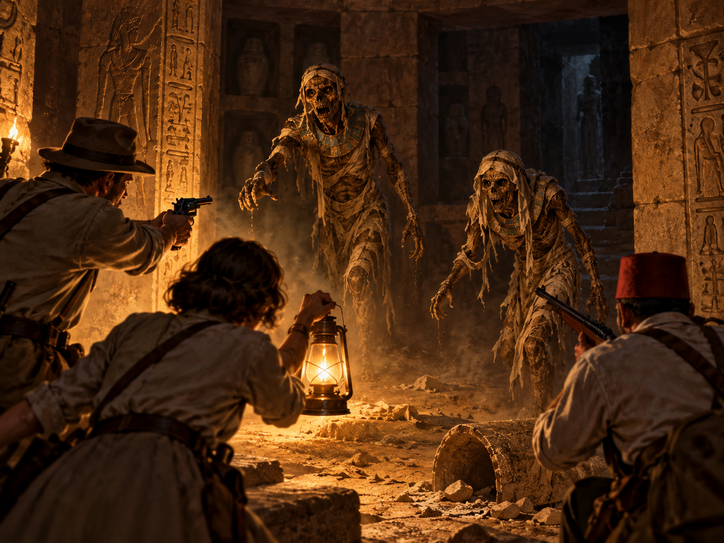
\includegraphics[width=\textwidth]{bilder/waechterleichname.png}\caption{Zwei uralte Wächterleichname schützen den Weg zur inneren Anlage.}\end{figure}
\begin{vorlesetextalle}
In einer länglichen Kammer stehen niedrige Steinsockel. Auf zweien liegen menschliche Gestalten, eingewickelt in dunkle, brüchige Leinenbinden. Harziger, trockener Geruch liegt in der Luft. Die Körper ruhen mit verschränkten Händen, den Kopf zur rückwärtigen Tür gewandt. Als Ihr Euch dieser nähert, raschelt Stoff. Eine der verdorrten Hände hebt sich.
\end{vorlesetextalle}
\begin{meisterinfo}
\textbf{Begegnung:} Zwei Wächterleichname, nicht gewöhnliche ägyptische Mumien. Sie können durch Waffen bekämpft oder umgangen werden: Engstelle nutzen, Sockel umwerfen, Ausgang blockieren, Ablenkung schaffen, Feuer an den Binden einsetzen. Keine weitere Gegnerwelle. \textbf{Stabilität:} 0/1W6 beim Anblick der sich bewegenden Toten.
\end{meisterinfo}
\subsection{Wächterleichnam -- Spielleitungswerte (je Exemplar)}
\begin{meisterinfo}
ST 70, KO 65, GR 60, GE 30, IN 10, MA 40. TP 12, Bewegung 5, Panzerung 2 (verhärtete Haut und Binden), Klauen 40\%, Schaden 1W4 + 1W4 Schadensbonus, Ausweichen 15\%, Stabilität 0/1W6. Die Wächter sind langsame, eigens für diese Szene entworfene Gegner. Sie reagieren auf Erschütterungen und den Durchgang zur inneren Kammer. \textbf{Belohnung für Planen:} Wer Nischen, Türrahmen, Seile oder mitgebrachte Geräte nutzt, kann einen Kampf vermeiden oder abkürzen.
\end{meisterinfo}
\section{4.9 -- Vor dem Portal der vier Wächter}
\begin{vorlesetextalle}
Ein breiter Gang führt tiefer in den Fels. Seine Wände sind ungewöhnlich glatt, die Bodenplatten dunkel und präzise gefügt. Geometrische Zeichen wiederholen sich entlang des Weges, manche ähneln dem Symbol auf dem sehenden Stein. Dann öffnet sich der Gang zu einem Vorraum. Vier niedrige Säulen stehen symmetrisch an den Wänden. Dahinter erhebt sich der breite, mit dunklen Zeichen versehene Durchgang zur eigentlichen Statuenhalle. Durch ihn dringt ein ungewöhnlich kalter Luftzug. Jenseits liegt ein gro\ss{}er Raum in tiefem Schatten; weiter hinten zeichnet sich ein gigantisches steinernes Tor ab. Zu Eurer Verwunderung ist der Boden auf dem Weg dorthin vollkommen frei von Staub.
\end{vorlesetextalle}
\begin{meisterinfo}
\textbf{Archäologie:} Vier symmetrische Säulen als Teil einer Konstruktion. \textbf{Verborgenes Erkennen:} Spuren eines älteren gewaltsamen Öffnungsversuchs. \textbf{Okkultismus:} Vier Positionen umschlie\ss{}en möglicherweise ein Zentrum. \textbf{Karte:} Die Gruppe steht vor dem von Flynn markierten Bereich der vier Statuen. \textbf{Szenenende:} Noch keine Lösung für die Statuen oder das Dimensionstor festlegen; das ist Gegenstand der nächsten Szene. Ermögliche Rückkehr, Rast und letzte Ausrüstungschecks.
\end{meisterinfo}

\chapter{Das Tor ins Nichts}
\noindent\textbf{Akt II, Szene 5:} Die vier Wächter, die andere Welt und die Flucht\\
\textbf{Ziel:} Flynn retten, den sehenden Stein in die Fassung der schwebenden Plattform einsetzen, den Übergang schlie\ss{}en und die zerfallende Anlage verlassen.

\begin{meisterinfo}
\textbf{Die Wahrheit:} Dr. Skorbinsk hielt das Auge für einen Schlüssel zur Öffnung. Tatsächlich dient der Stein als Siegel einer uralten Grenzvorrichtung. Seine Entnahme lie\ss{} den Durchgang instabil werden; die vier Statuen begrenzen ihn. Zeitliche Echos erklären die Karte in Arkham, die Erscheinung Yusufs und die anomalen Zustände im Carlson-Haus. Die genauen Gesetze bleiben auch nach dem Finale unbegreiflich. \textbf{Flynn} lebt auf der Plattform und ist rettbar. \textbf{Skorbinsk} starb in der Statuenhalle. \textbf{Der Stein bleibt nach dem Verschlie\ss{}en endgültig in der Plattform zurück und geht mit der anderen Dimension verloren. Er wird nicht wiedergefunden und verwandelt sich nicht in ein Älteres Zeichen.} Die Abbildungen zeigen Spielleitungsillustrationen, keine zwingend wortwörtliche Architektur.
\end{meisterinfo}

\section{5.1 -- Die Halle der vier Wächter}
\begin{vorlesetextalle}
Ihr tretet durch den dunklen Durchgang in eine Halle von gewaltigen Ausma\ss{}en. Vier hohe steinerne Gestalten stehen um eine kreisförmige Bodenfläche; ihre glatten Gesichter und langen Stäbe wirken weder ägyptisch noch menschlich vertraut. Ihre Blicke richten sich über die Mitte hinweg auf ein riesiges, weit geöffnetes Tor. Dahinter ist keine Mauer, kein weiterer Raum, sondern eine Dunkelheit mit fernen, unsteten Lichtpunkten. Eure Lampen vermögen ihre Tiefe nicht zu ergründen.
\end{vorlesetextalle}
\begin{meisterinfo}
\textbf{Archäologie:} Die Statuen sind älter als die ägyptisch anmutenden Ergänzungen. \textbf{Verborgenes Erkennen:} Linien unter ihren Sockeln laufen auf das Tor zu. \textbf{Okkultismus:} Die vier Wächter begrenzen einen Übergang, statt selbst anzugreifen. \textbf{Idee:} Skorbinsks Skizze mit vier Markierungen zeigt genau diese Anordnung. Das Tor ist bereits geöffnet; es braucht kein zusätzliches Öffnungsritual. \textbf{Fundabsicherung:} Falls der sehende Stein zuvor nicht aufgenommen wurde, liegt er deutlich sichtbar unmittelbar vor der Schwelle. Er kann ohne Probe genommen werden.
\end{meisterinfo}

\section{5.2 -- Dr. Skorbinsks letztes Zeugnis}
\begin{vorlesetextalle}
Am Sockel einer Statue sitzt ein regloser Mann. Kleidung und Gesicht sind von Staub bedeckt; neben seiner Hand liegen verstreute Blätter und eine zerbrochene Brille. Ihr erkennt Dr. Skorbinsk. Seine Augen starren unverwandt auf das offene Tor. Auf einem der Blätter stehen hastig geschriebene Worte: \glqq{}Ich dachte, es sei ein Schlüssel. Ich verstand nicht, dass es ein Siegel war. Vier halten die Grenze. Das Auge schlie\ss{}t.\grqq{}
\end{vorlesetextalle}
\begin{meisterinfo}
\textbf{Medizin:} Skorbinsk ist tot, ohne klare äu\ss{}ere Todesursache. \textbf{Stabilität:} 0/1W3 STA beim Auffinden. \textbf{Folgerung:} Stein und vier Wächter gehören zusammen; der Abschluss findet jenseits des Tores statt. Skorbinsk ist nicht als Kampfgegner vorgesehen.
\end{meisterinfo}

\section{5.3 -- Blick durch das Tor}
\begin{figure}[htbp]\centering
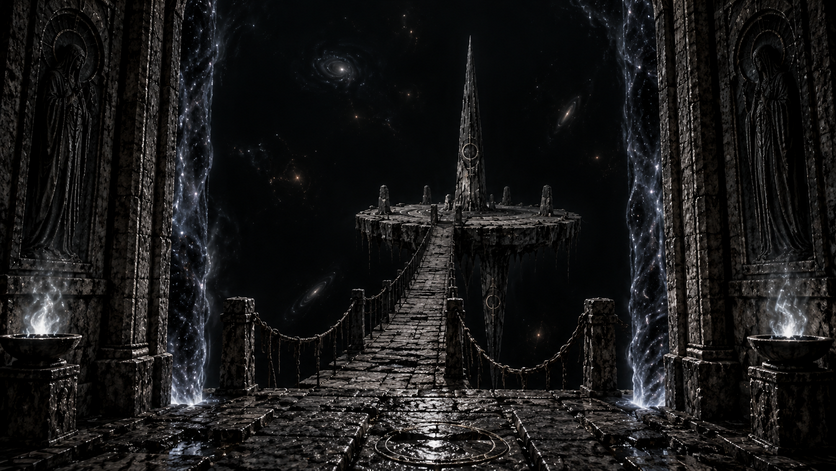
\includegraphics[width=\textwidth]{bilder/finale-tor-im-nichts.png}
\caption{Blick von der steinernen Schwelle zur frei schwebenden Plattform im Nichts.}
\end{figure}
\begin{vorlesetextalle}
Durch das Tor führt eine schmale Hängebrücke aus dunklen Steinplatten, gehalten von schweren Ketten. Sie endet an einer etwa fünf Meter breiten, kreisrunden Plattform, die frei in einer endlosen Dunkelheit schwebt. Aus ihrer Mitte erhebt sich eine steinerne Nadel; eine zweite, ebenso spitze ragt von ihrer Unterseite hinab. Weit entfernt funkeln Lichtpunkte wie Sterne, doch sobald Ihr sie fixiert, scheinen sich ihre Entfernungen zu verändern. Kein Horizont, kein Oben, kein Unten gibt Euch Halt. Ein bedrückendes Gefühl breitet sich in Eurer Brust aus, als wäre die Unendlichkeit selbst zu schwer für Eure Gedanken.
\end{vorlesetextalle}
\begin{meisterinfo}
\textbf{Stabilität:} Beim ersten ungeschützten Blick 1/1W6 STA. \textbf{Schwelle:} Der Atem ist möglich; die Luft folgt hier offenbar eigenen Regeln. Die Brücke ist begehbar und trägt die Gruppe, auch wenn sie schwankt. \textbf{Orientierung oder Idee:} Wer sich auf einzelne Schritte statt auf die Ferne konzentriert, kann ruhiger vorankommen.
\end{meisterinfo}

\section{5.4 -- Die Brücke und ihre Rückseite}
\begin{vorlesetextalle}
Die Platten schwingen leicht unter Euren Schuhen. Je weiter Ihr geht, desto unwirklicher wird die Entfernung zur Plattform. Als Ihr zurückblickt, erkennt Ihr die Rückseite des steinernen Tores frei im Nichts. Die Statuenhalle ist von hier aus verschwunden; allein der Rahmen hängt ohne Stütze in der grenzenlosen Leere. Für einen schrecklichen Moment fragt Ihr Euch, ob jenseits der Schwelle überhaupt noch Eure Welt existiert.
\end{vorlesetextalle}
\begin{meisterinfo}
\textbf{Stabilität:} Beim erstmaligen Erkennen der frei schwebenden Rückseite 0/1W3 STA. Nach jeweils weiteren fünf Minuten auf Brücke oder Plattform 0/1W3 STA; nicht in jeder Runde wiederholen. \textbf{Interaktion:} Orientierung (Rhythmus der Schritte), Psychologie (Gefährten beruhigen), Klettern und Stärke (Hilfe bei einem Stolpern). Fehlwürfe kosten Zeit oder verursachen eine brenzlige Lage, nicht automatisch einen Absturz. \textbf{Rückweg:} Trotz optischer Verwirrung bleibt der Übergang erreichbar.
\end{meisterinfo}

\section{5.5 -- Flynn Carlson auf der Plattform}
\begin{vorlesetextalle}
Die Plattform besteht aus ebenem schwarzem Stein, in den konzentrische Linien eingearbeitet wurden. Zwischen ihnen befindet sich eine handtellergro\ss{}e Vertiefung mit dem Zeichen des Auges. Am Fu\ss{} der aufragenden Nadel kauert ein erschöpfter Mann in zerrissener Kleidung. Er hebt langsam den Kopf. \glqq{}Seid Ihr wirklich hier? Oder seid Ihr wieder eine Erscheinung?\grqq{} Seine Stimme ist kaum mehr als ein Flüstern. \glqq{}Ich bin Flynn Carlson. Wie lange bin ich hier?\grqq{}
\end{vorlesetextalle}
\begin{meisterinfo}
\textbf{Flynn lebt:} Für ihn könnten subjektiv nur Tage vergangen sein. \textbf{Erste Hilfe/Medizin:} Schwäche, Durst und Desorientierung; er ist gestützt transportfähig. \textbf{Psychologie:} Ruhiges Ansprechen hilft ihm, bei der Gruppe zu bleiben. Er kann berichten, dass Skorbinsk das Artefakt als Schlüssel verstand und dass nach dem Öffnen fremde Wesen erschienen. Von Helenas Tod wei\ss{} er nichts; ob die Ermittler ihn hier darüber informieren, entscheiden die Spieler. \textbf{Sicherheit:} Er darf gerettet werden, ohne dass ein Einzelwurf das Schicksal automatisch festlegt.
\end{meisterinfo}

\section{5.6 -- Das Siegel wird eingesetzt}
\begin{vorlesetextalle}
Als Ihr den Stein mit dem Auge über die Vertiefung hebt, beginnt seine Gravur fahl zu leuchten. Das Artefakt gleitet in die Fassung und sitzt darin vollkommen fest. Silberne Linien breiten sich über den Boden aus; die beiden Steinnadeln beginnen zu vibrieren. Um Euch ziehen sich ferne Lichtpunkte zusammen. Dann hört Ihr eine Stimme, die von keinem bestimmten Ort zu kommen scheint: \glqq{}Endlich.\grqq{}
\end{vorlesetextalle}
\begin{meisterinfo}
\textbf{Keine Probe notwendig:} Das Einsetzen ist die Lösung. Eine gelungene Idee- oder Okkultismusprobe darf zuvor einen Hinweis geben. \textbf{Unwiderruflich:} Der Stein verschmilzt mit der Fassung und ist nicht mehr herauszulösen. Er bleibt in der sich auflösenden jenseitigen Konstruktion und ist endgültig verloren. Mit dem Einsetzen beginnt der Verschluss, zugleich aber der Zerfall der Anlage. \textbf{Nicht den Sieg durch eine weitere Pflichtprobe entwerten.}
\end{meisterinfo}

\section{5.7 -- Bast, die Hüterin der Grenze}
\begin{vorlesetextalle}
Vor Euch flimmert die Dunkelheit. Eine schlanke Gestalt tritt hervor, von beinahe menschlicher Haltung, doch mit dem Haupt und den Augen einer Katze. Ein schlichtes Gewand umhüllt ihren Körper. Sie betrachtet die leuchtende Fassung. \glqq{}Die Grenze wird wiederhergestellt. Ihr habt geschlossen, was nicht hätte offen stehen dürfen. Durch diese Schwelle kamen Dinge in Eure Welt, die dort keinen Platz haben. Wäre sie geblieben, wären andere gefolgt.\grqq{} Ein gewaltiges Grollen erschüttert die Plattform. \glqq{}Die Verbindung zerfällt nun, und mit ihr die Steine, die sie halten. Geht. Nehmt den Lebenden mit. Kehrt zurück, ehe der Weg vergeht.\grqq{} Ihre Augen verweilen einen letzten Moment auf Euch. \glqq{}Nicht alles, was Euch sieht, wünscht Euch Schaden.\grqq{} Dann verblasst ihre Erscheinung.
\end{vorlesetextalle}
\begin{meisterinfo}
\textbf{Bast ist keine Gegnerin.} Sie erläutert nur das unbedingt Nötige: Tor offen, fremde Wesen (darunter der Dhole), Gefahr für die Welt, jetzt Verschluss und Kollaps. Die Vision soll kurz bleiben. Kein zusätzlicher Stabilitätswurf nötig. \textbf{Stein:} Bast gibt ihn nicht zurück und verspricht auch keinen Ersatz.
\end{meisterinfo}

\section{5.8 -- Rückweg über die brechende Brücke}
\begin{vorlesetextalle}
Ein Krachen läuft durch die Nadel. Die Plattform schwankt und ein Stück Fels bricht an ihrem Rand ab, ohne irgendwo aufzuschlagen. Die Ketten der Brücke spannen sich knarrend. Am fernen Ende scheint das Tor mal die Statuenhalle, mal nur eine dunkle Oberfläche zu zeigen. Ein weiterer Ruck zwingt Euch, Halt zu suchen. Ihr müsst zurück -- und Flynn kann kaum allein gehen.
\end{vorlesetextalle}
\begin{meisterinfo}
\textbf{Drei Phasen:} (1) Flynn aufrichten und die Plattform verlassen (Stärke, Erste Hilfe, Teamarbeit); (2) über die schwankende Brücke (Klettern, Springen, Verborgenes Erkennen, Seilsicherung); (3) geschlossen durch das Tor gelangen (Orientierung, Absprachen, Rettungsversuche). Erfolgreiche clevere Ideen zählen wie Proben. Fehlschläge kosten Zeit, Ausrüstung oder verursachen kleinere Verletzungen. Eine tödliche Konsequenz nur nach deutlich angekündigten Risiken und mehrfachen Fehlschlägen. Die Erkundung soll nicht mit einer zufälligen Einzelprobe enden.
\end{meisterinfo}

\section{5.9 -- Das Tor wird zu nacktem Stein}
\begin{vorlesetextalle}
Ihr stolpert durch die Schwelle zurück auf festen Boden. Hinter Euch hängt die Brücke noch im Nichts, doch ihre Konturen werden blass. Die Sterne verlöschen, die Plattform und ihre Nadeln zerflie\ss{}en im Dunkel. Wo eben noch unendlicher Raum lag, wird eine kahle Felswand sichtbar. Schlie\ss{}lich steht das Tor vor nichts anderem als festem Stein. Dann splittert eine der vier Statuen. Das Krachen weiterer Risse erfüllt die Halle. Gewaltige Blöcke stürzen zu Boden.
\end{vorlesetextalle}
\begin{meisterinfo}
Die vier Statuen waren Grenzwächter, keine Kampfgegner. Mit dem geschlossenen Übergang verlieren sie ihre Funktion und zerfallen. Das Tor bleibt auf dieser Seite nur ein bedeutungsloser Rahmen vor einer Felswand. Der Stein ist nicht hier, sondern im verlorenen Jenseits.
\end{meisterinfo}

\section{5.10 -- Flucht aus den zerfallenden Katakomben}
\begin{vorlesetextalle}
Die Halle bebt. Staub und Steinsplitter regnen von der Decke. Ihr eilt durch bekannte Gänge, doch an mehreren Stellen versperren herabgestürzte Blöcke den Weg. Hinter Euch donnert ein tiefer Einsturz durch die Anlage. Aus der Ferne klingt das Brechen schwerer Gesteinsmassen wie ein Gewitter unter der Erde. Vor Euch liegt irgendwo der Ausgang zur Wüste.
\end{vorlesetextalle}
\begin{meisterinfo}
\textbf{Gruppenherausforderung:} Fünf Erfolge vor drei schweren Rückschlägen. Jede Figur beschreibt einen sinnvollen Beitrag; nicht immer denselben Wurf wiederholen. Geeignet: Orientierung mit Flynns Karte, Stärke zum Freiräumen, Klettern/Springen, Verborgenes Erkennen für instabile Decken, Erste Hilfe für Verletzte, Psychologie gegen Panik. Erfolge schaffen echte Fortschritte. Fehlschläge führen zu verlorener Zeit, verlorener Ausrüstung oder einer Verletzung. Bei drei Rückschlägen folgt ein letzter schwieriger Ausgang statt automatischer Gruppenvernichtung. Flynn braucht Hilfe, darf aber bei kluger Zusammenarbeit mitgerettet werden.
\end{meisterinfo}

\section{5.11 -- Wieder unter der Sonne}
\begin{vorlesetextalle}
Endlich erscheint Tageslicht. Ihr stolpert aus der Felsöffnung in warme, trockene Luft. Hinter Euch knicken hölzerne Stützen ein, ein tiefes Donnern läuft durch den Berghang. Geröll stürzt herab und verschüttet den Eingang vollständig. Dann legt sich der Staub. Wo die Expedition einst die unterirdische Anlage freigelegt hatte, liegt nur noch gewöhnlicher Stein. Über Euch spannt sich ein blauer Himmel. Zum ersten Mal seit Langem fühlt sich die Welt wieder vertraut an.
\end{vorlesetextalle}

\chapter*{Epilog -- Was bleibt}
\addcontentsline{toc}{chapter}{Epilog -- Was bleibt}
\begin{vorlesetextalle}
Die Tage nach Eurer Flucht sind erfüllt von Rückreisevorbereitungen, Erschöpfung und Gesprächen über das Unbegreifliche. Flynn Carlson hat die Katastrophe überlebt. Doch die Nachricht vom Tod seiner Frau liegt schwer auf ihm, und seine Erinnerungen an die schwebende Plattform folgen ihm bis in den Schlaf. Als Ihr Arkham wieder erreicht, bleibt der Universität nur Euer Bericht. Die Beweise liegen verschüttet unter ägyptischem Fels, und manches scheint selbst im Rückblick kaum möglich. Ihr habt das Tor geschlossen -- und den sehenden Stein mit ihm verloren. Was immer jene Grenze bewachte, besteht nun wieder jenseits menschlicher Reichweite.
\end{vorlesetextalle}
\begin{meisterinfo}
\textbf{Abschluss:} Flynn kann nach Arkham zurückkehren und Helenas Verlust betrauern. Präsident Garmond erhält die Nachricht vom gescheiterten Ausgrabungsprojekt und der Rettung seines Mitarbeiters. Der sehende Stein ist \emph{endgültig verloren}; es gibt \emph{keine} spätere Rückkehr, keine Verwandlung in ein Älteres Zeichen und keinen Artefakt-Bonus. Der übernatürliche Schrecken ist vorerst eingedämmt, nicht vollends erklärt. Wenn gewünscht, kann die Gruppe für den Erfolg eine angemessene Stabilitätsbelohnung erhalten (nach Regelwerksausgabe und Spielleitungsermessen).
\end{meisterinfo}

\end{document}
